\appendix

\section{Voting Interface Breakdown}\label{apdx:relatedVoting}
Compared to digital survey interfaces, there exists a rich literature on voting interfaces, which we argue is a special type of survey interface. We categorize these related works into three main categories detailed below:

\paragraph{Designs that shifted voter decisions: } For example, states without straight-party ticket voting~(where voters can select all candidates from one party through a single choice) exhibited higher rates of split-ticket voting~\cite{engstrom2020politics}. Another example from the Australian ballot showing incumbency advantages is where candidates are listed by the office they are running for, with no party labels or boxes.
\paragraph{Designs that influenced errors: } Butterfly ballots increased voter errors because voters could not correctly identify the punch hole on the ballot. Splitting contestants across columns increases the chance for voters to overvote~\cite{quesenberyOpinionGoodDesign2020}. On the other hand, \textcite{everettElectronicVotingMachines2008} showed the use of incorporating physical voting behaviors, like lever voting, into graphical user interfaces.

\paragraph{Designs that incorporated technologies: } Other projects like the Caltech-MIT Voting Technology Project have sparked research to address accessibility challenges, resulting in innovations like EZ Ballot~\cite{leeUniversalDesignBallot2016}, Anywhere Ballot~\cite{summers2014making}, and Prime III~\cite{dawkinsPrimeIIIInnovative2009}. In addition, \textcite{gilbertAnomalyDetectionElectronic2013} investigated optimal touchpoints on voting interfaces, and \textcite{conradElectronicVotingEliminates2009} examined zoomable voting interfaces.

% *********************************************************** %
\section{Interface design process}\label{apdx:design}
In this section, we outline the design process leading to our final interface. As mentioned in the paper, our design iteration began from existing QV applications in the wild.

\begin{figure}[ht]
    \centering
    \begin{subfigure}[b]{0.54\textwidth}
        \centering
        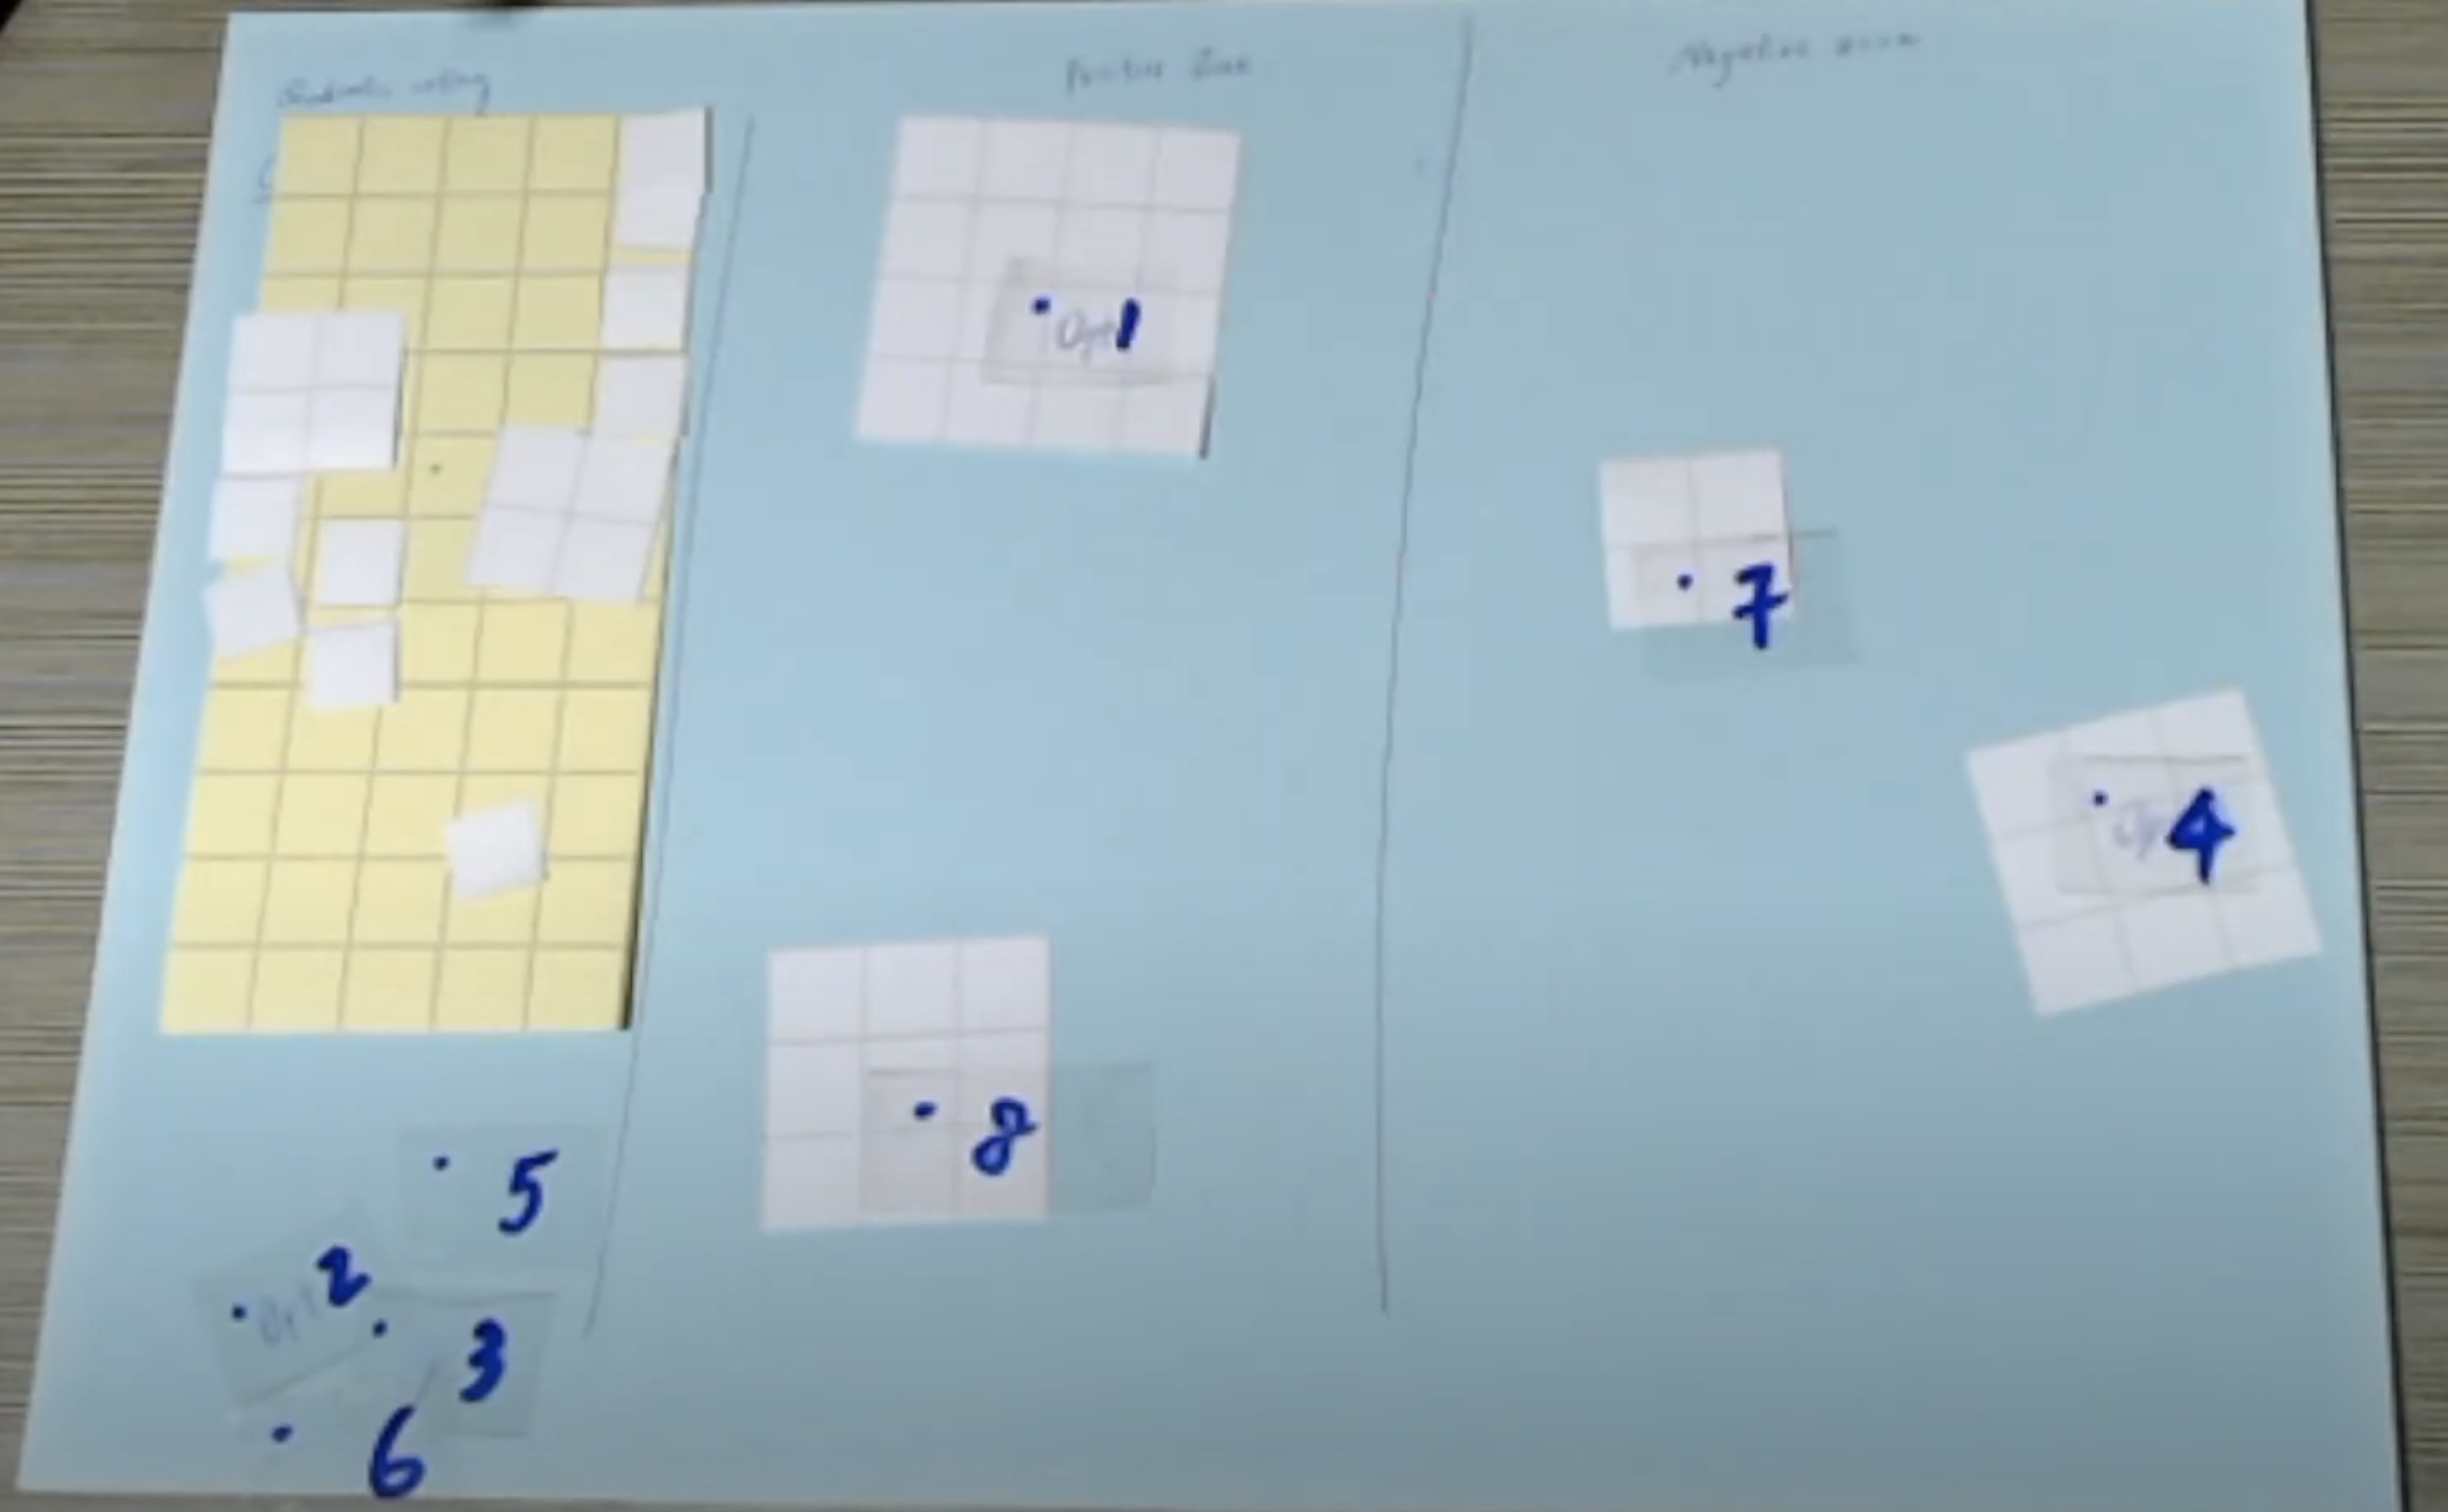
\includegraphics[width=\textwidth]{content/image/prototypes/1.2_paper_qv_single.png}
        \caption{In this paper prototype, issues are denoted by different numbers that appear on mouseover. Pretest respondents can move options anywhere in the two sections of the interface, one denoting positive and one negative. The blocks represent the cost for each option, with no indication of the number of current votes. The credits are shown in the yellow box on the left.}
        \Description{An image of a paper prototype showing different sections for respondents to interact with. On the left side, a yellow grid contains small white squares, some of which are stacked and scattered outside the grid. The middle section labeled "Positive Zone" contains a large white square with a grid, labeled "Opt 1". The right section, labeled "Negative Zone," contains two white squares, each with grids, labeled with numbers 7 and 4. Additional small white squares labeled with numbers 2, 3, 5, 6, and 8 are positioned around the prototype. The yellow box on the left represents available credits.}
        \label{fig:horizontal_paper}
    \end{subfigure}
    \hfill
    \begin{subfigure}[b]{0.42\textwidth}
        \centering
        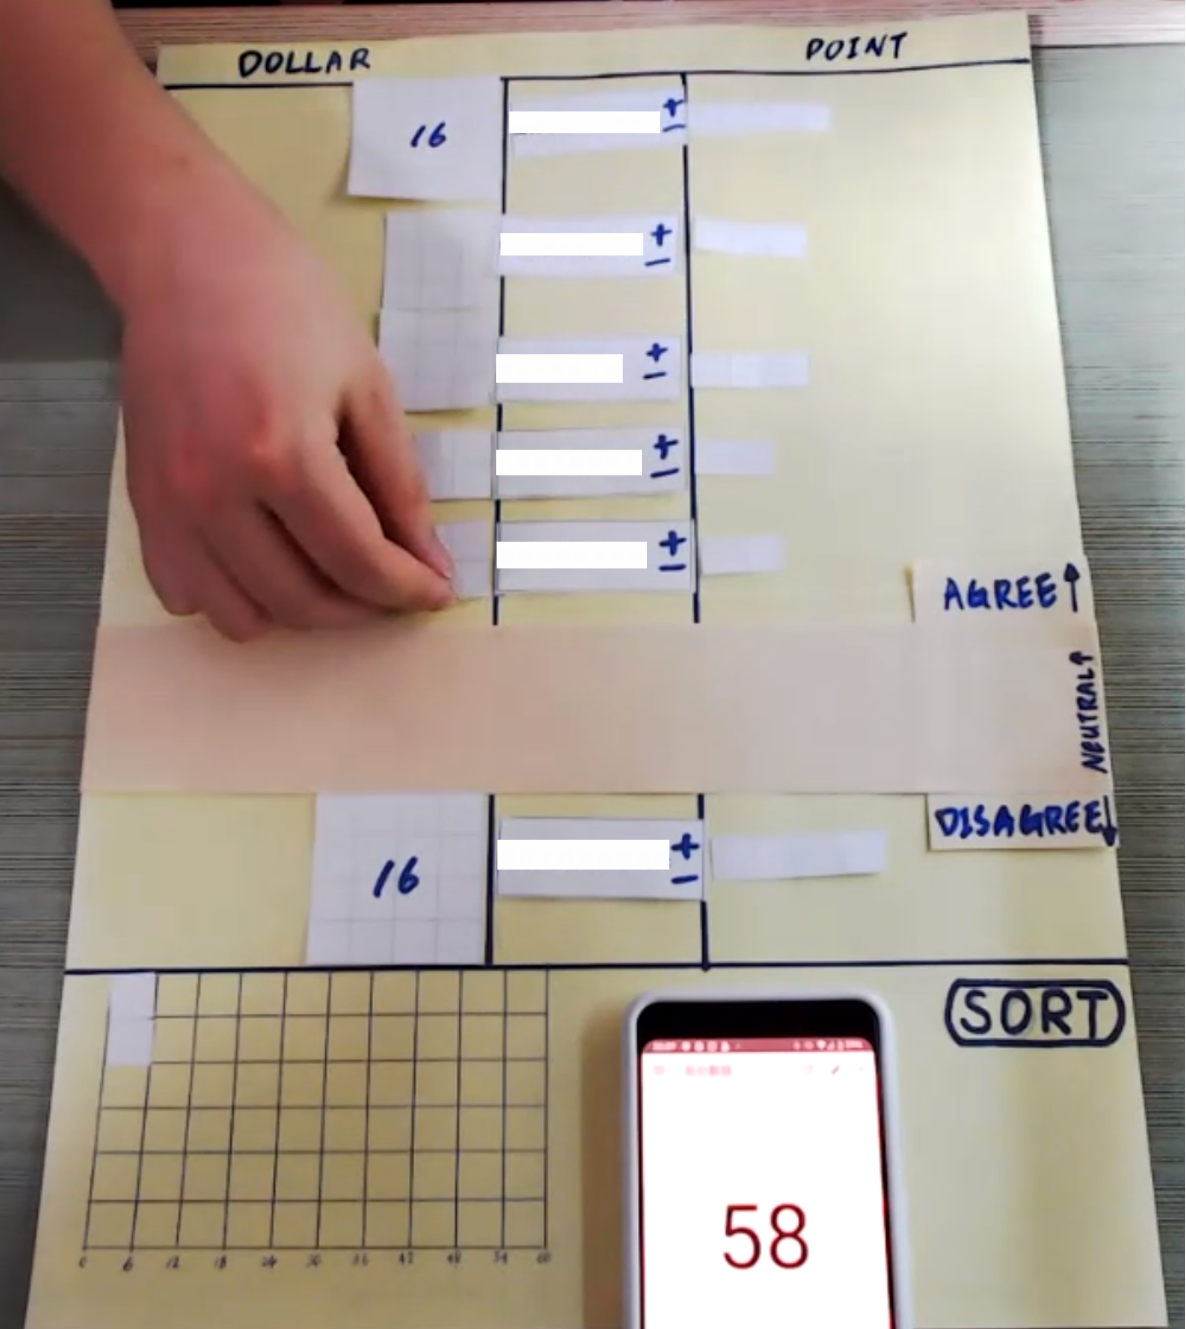
\includegraphics[width=\textwidth]{content/image/prototypes/1_paper_qv_single.png}
        \caption{This paper prototype separates the positive and negative areas with a 'band' at the center. Undecided options are placed inside this band. The cost and the votes on both sides of the interface are denoted by small blocks. The budget is shown in the yellow box below the interface with a numerical counter.}
        \Description{A paper prototype interface where a person's hand is interacting with blocks. The prototype separates positive and negative areas using a wide horizontal band in the center, which holds undecided options. On the left side of the band, a column labeled "Dollar" shows a block marked with the number 16. On the right side, under a column labeled "Point," several rows have small blocks with plus and minus signs, indicating positive and negative areas. At the bottom left, a yellow box with a grid shows the available budget, marked with the number 16. A smartphone in the bottom right corner displays the number 58.}
        \label{fig:vertical_paper}
    \end{subfigure}
    \caption{Initial paper prototypes designed for QS interface}
    \Description{This figure contains two subfigures showing two different paper prototypes.}
    \label{fig:qv_paper}
\end{figure}

\subsection{Prototype 1: Ranking-Vote}
Considering that relative preference is often through ranking items, we tested whether ranking options before voting would help establish an individual's relative preference in our prototype 1. This prototype allowed respondents to reposition options before voting. Pretests revealed that respondents rarely moved the options and questioned the necessity of full ranking, as it did not influence their QS submission. Additionally, many were unaware that options were draggable until shown. This insight indicates that full ranking is unnecessary for establishing relative preferences. Therefore, we decided to ask respondents to select a subset of options instead of requiring a full rank among all options.

\begin{figure}[ht]
    \centering
    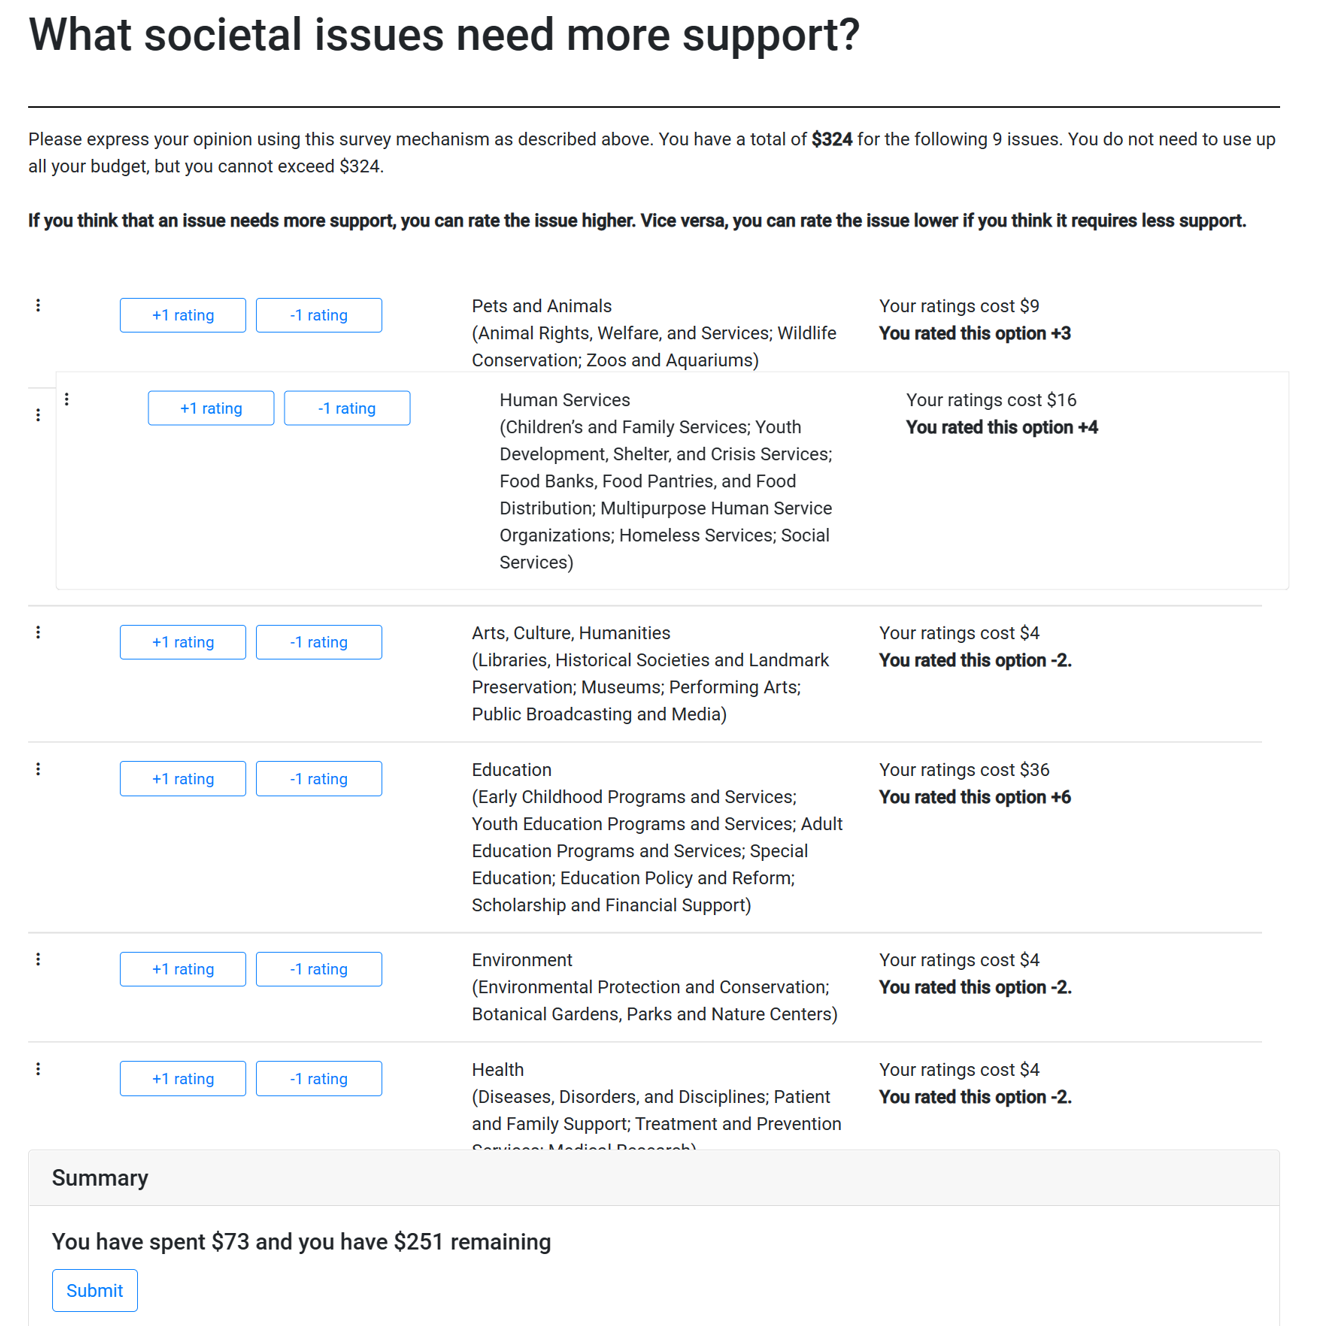
\includegraphics[width=0.4\textwidth]{content/image/prototypes/2_ranking.png}
    \caption{A Ranking-Vote Prototype: The goal of this prototype is to test whether ranking options prior to voting help establish an individual's relative preferences and reduce effort when voting. Each option is draggable to position in a specific location amongst the full list of options. Votes can be updated using the buttons to the right of the interface with vote count and costs to the right of the interface. A summary box is placed sticky to the bottom of the screen.}
    \Description{A web interface showing a survey titled "What societal issues need more support?" The interface presents several societal issues in a list format, each with buttons labeled "+1 rating" and "-1 rating" to adjust the ratings. For example, the issue "Pets and Animals" shows a rating cost of \$9 with a +3 rating, and "Human Services" shows a rating cost of \$16 with a +4 rating. The remaining issues include Arts, Culture, Humanities, Education, Environment, and Health, each with their respective ratings and costs. At the bottom of the page is a summary box displaying the total spent (\$73) and the remaining balance (\$251). A "Submit" button is positioned below the summary.}
    \label{fig:qv_rank}
\end{figure}

\begin{figure}[ht]
    \centering
    \begin{subfigure}[b]{0.47\textwidth}
        \centering
        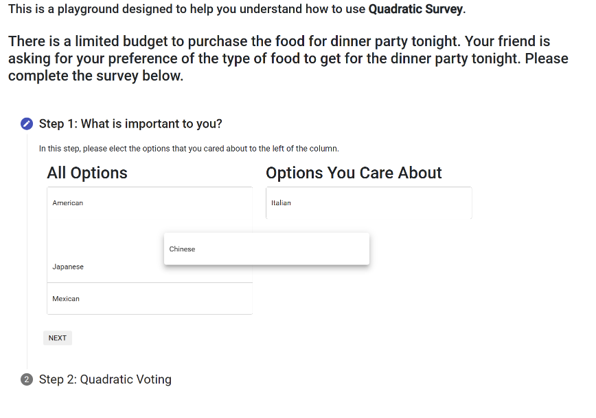
\includegraphics[width=0.9\textwidth]{content/image/prototypes/3.1_selecting.png}
        \caption{Options are dragged and dropped to the 'Option You Care About' box.}
        \Description{A web interface showing the first step of a quadratic voting prototype. The screen is titled "What is important to you?" On the left, under "All Options," a list of food types is displayed, including American, Japanese, and Mexican. One option, "Chinese," is being dragged to the right column labeled "Options You Care About," which already includes "Italian." A "Next" button appears at the bottom of the interface.}

        \label{fig:qv_select_selection}
    \end{subfigure}
    \hfill
    \begin{subfigure}[b]{0.47\textwidth}
        \centering
        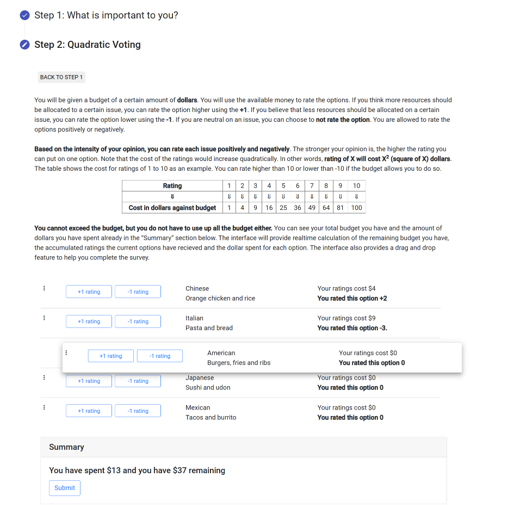
\includegraphics[width=0.9\textwidth]{content/image/prototypes/3.2_selecting_2.png}
        \caption{The previous step collapses showing all voting options.}
        \Description{The second step of a quadratic voting prototype showing a list of food options for voting. The voting interface displays food items such as Chinese, Pasta and bread, and American. Next to each item are "+1 rating" and "-1 rating" buttons for adjusting votes. Each option also shows the cost of votes, and a summary box at the bottom displays the amount spent (\$13) and the remaining balance (\$37).}

        \label{fig:qv_select_vote}
    \end{subfigure}
    \caption{A Select-then-Vote Prototype: The goal of this prototype is to nudge participants to focus on a subset of options to vote, rather than ranking all of them. This prototype introduces a two-step voting process. As shown in Fig.~\ref{fig:qv_select_selection}, the first step involves selecting options for further consideration. Important options are placed at the top of the list for voting shown in Fig.~\ref{fig:qv_select_vote}, but options can be placed anywhere on the list if desired. The rest of the controls remain the same as the previous prototype.}
    \Description{A two-step quadratic voting prototype interface. In the first step (Subfigure 1), users drag and drop food options from a list on the left, such as American and Mexican, to the "Options You Care About" box on the right. In the second step (Subfigure 2), users vote on their selected options by adjusting the ratings using "+1 rating" and "-1 rating" buttons. A summary at the bottom shows the total amount spent and remaining balance.}

    \label{fig:qv_select}
\end{figure}

\subsection{Prototype 2: Select-then-Vote}
Based on feedback from Prototype 1, instead of \textit{allowing} individuals to rank options, Prototype 2 implemented a two-phase process that \textit{intentionally} asks respondents to select options to express opinions before voting. As shown in Figure~\ref{fig:qv_select}, survey respondents selected their preferred options (Figure~\ref{fig:qv_select_selection}), and the interface positioned these options at the top of the list for voting (Figure~\ref{fig:qv_select_vote}). We identified several issues during the prototype 2 pretest: many respondents marked most options as 'options they care about,' which undermined the design's purpose. Additionally, the lack of clear distinction between selected and unselected options confused respondents about the necessity of Step 1. Thus, we need a clearer distinction and connection between the two phases to effectively construct relative preferences.

\begin{figure}[ht]
    \centering
    \begin{subfigure}[b]{0.45\textwidth}
        \centering
        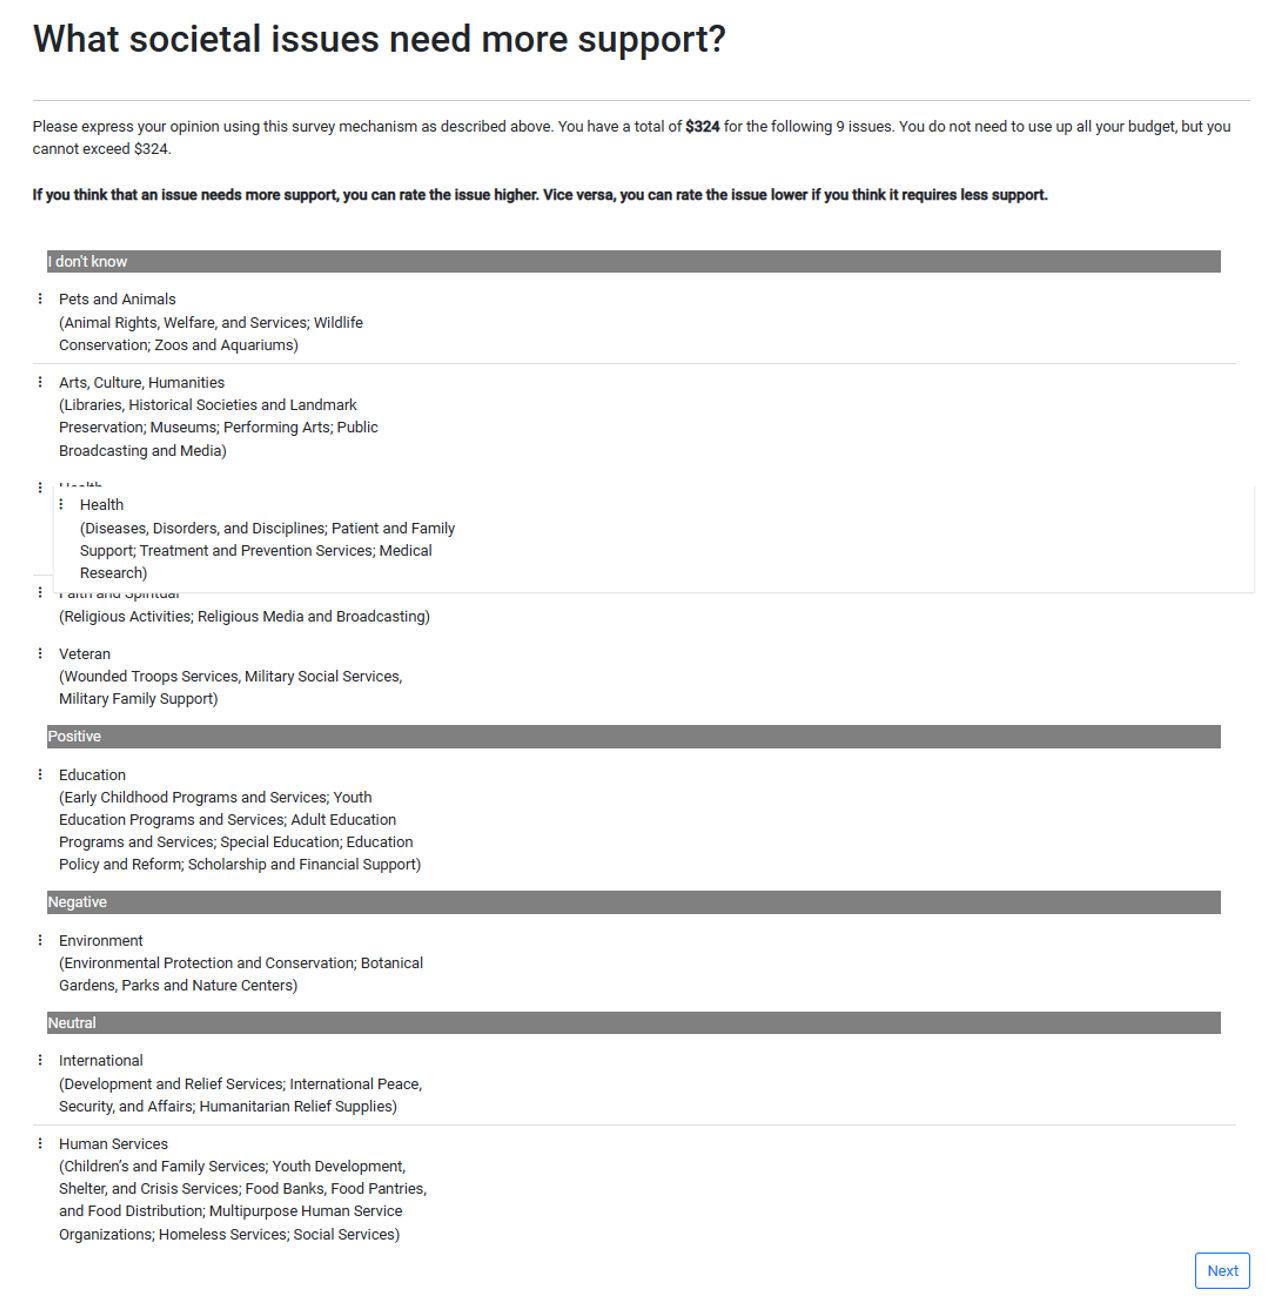
\includegraphics[width=\textwidth]{content/image/prototypes/4.1_grouping.png}
        \caption{The Organization Interface: Options are shown initially in the first bin labeled as `I don't know.' Survey respondents can then drag and drop these options into the latter bins: Lean Positive, Lean Neutral, or Lean Negative. Only the details of each option are shown on this interface.}
        \Description{A web interface displaying a survey titled "What societal issues need more support?" Initially, all options are placed in the first bin labeled "I don't know." The listed options include Pets and Animals, Arts, Culture, Humanities, Health, Veterans, and others. Each option is accompanied by a brief description. Below the "I don't know" bin are three other bins: "Positive," "Negative," and "Neutral." Survey respondents can drag and drop options into these bins based on their preferences. A "Next" button is located at the bottom right corner of the interface.}
        \label{fig:qv_org_p1}
    \end{subfigure}
    \hfill
    \begin{subfigure}[b]{0.45\textwidth}
        \centering
        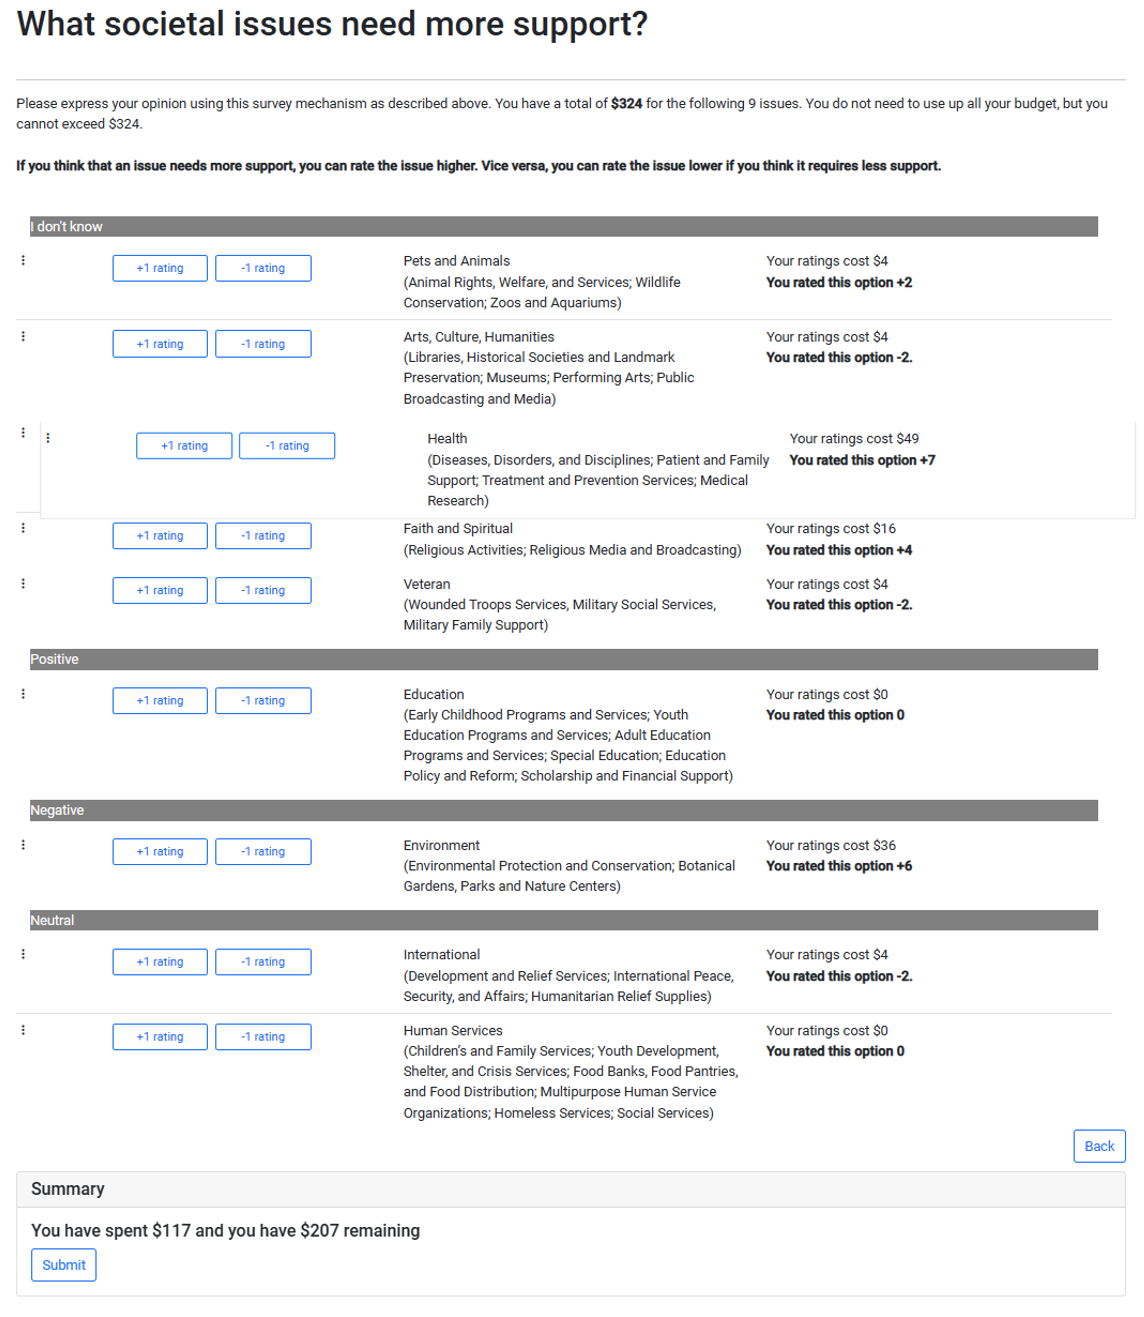
\includegraphics[width=\textwidth]{content/image/prototypes/4.2_grouping_vote.png}
        \caption{The Voting Interface: Voting controls appear on the left side of each option, showing the current votes and associated costs on the right. A budget summary is stuck at the bottom of the screen.}
        \Description{A web interface displaying a survey titled "What societal issues need more support?" Each option in the list has voting controls, with "+1 rating" and "-1 rating" buttons appearing on the left side of each issue. The issues are grouped into categories such as "I don't know," "Positive," "Negative," and "Neutral." To the right of each issue, the cost of the rating is shown along with the number of votes cast. For example, "Pets and Animals" has a rating cost of \$4 with a +2 rating, while "Health" has a rating cost of \$49 with a +7 rating. At the bottom of the page, a summary box shows the total amount spent (\$117) and the remaining balance (\$207), with a "Submit" button below it.}

        \label{fig:qv_org_p2}
    \end{subfigure}
    \caption{Organize-then-Vote Prototype: The goal of this prototype is to encourage participants to derive finer grain categories among options before voting. Survey respondents first organize their thoughts into categories and then vote on the options.}
    \Description{The figure shows an Organize-then-Vote prototype with two main steps. In the first step, the left figure, users organize options by dragging and dropping them into different categories: "I don't know," "Positive," "Neutral," or "Negative." In the second step, the right figure, users vote on these organized options using "+1 rating" and "-1 rating" buttons, with voting costs and current ratings displayed. A summary section shows the total spent and remaining budget.}


    \label{fig:qv_org}
\end{figure}

\subsection{Prototype 3: Organize-then-Vote}
Figure~\ref{fig:qv_org} shows the last prototype where we built on the previous takeaway by providing finer-grain groupings and creating a clear connection between option organization and voting position. Specifically, we provided three categories: Lean Positive, Lean Negative, and Lean Neutral. Initially, respondents see all options under the section labeled 'I don't know,' which includes only the option descriptions. We ask respondents to move these options into the categories below. Voting controls and information appear on each option once respondents move to the subsequent page, forming a clear connection between option groups, positions, and voting controls.

Feedback indicated that survey respondents are comfortable with the two-phase organize-then-vote design, demonstrating it as a central strategy for our interface development. However, several areas for enhancement were identified: First, the dragging and dropping mechanism in the organization phase is cumbersome and may inadvertently suggest a ranking process, contrary to our intentions. Second, placing unorganized options at the top of the voting list is counterintuitive. Third, the voting controls are disconnected from the option summaries, dividing attention between the left and right sides of the screen. These insights guided refinements in the final two-phase interface, adhering to the two-phase organize-then-vote design framework.

% *********************************************************** %
\section{List of Options}
\label{sec:charityList}
We provide the full list of options presented on the survey.

\begin{itemize}
    \item \textbf{Animal Rights, Welfare, and Services:} Protect animals from cruelty, exploitation and other abuses, provide veterinary services and train guide dogs.
    \item \textbf{Wildlife Conservation:} Protect wildlife habitats, including fish, wildlife, and bird refuges and sanctuaries.
    \item \textbf{Zoos and Aquariums:} Support and invest in zoos, aquariums and zoological societies in communities throughout the country.
    \item \textbf{Libraries, Historical Societies and Landmark Preservation:} Support and invest public and specialized libraries, historical societies, historical preservation programs, and historical estates.
    \item \textbf{Museums:} Support and invest in maintaining collections and provide training to practitioners in traditional arts, science, technology, and natural history.
    \item \textbf{Performing Arts:} Support symphonies, orchestras, and other musical groups; ballets and operas; theater groups; arts festivals; and performance halls and cultural centers.
    \item \textbf{Public Broadcasting and Media:} Support public television and radio stations and networks, as well as providing other independent media and communications services to the public.
    \item \textbf{Community Foundations:} Promote giving by managing long-term donor-advised charitable funds for individual givers and distributing those funds to community-based charities over time.
    \item \textbf{Housing and Neighborhood Development:} Lead and finance development projects that invest in and improve communities by providing utility assistance, small business support programs, and other revitalization projects.
    \item \textbf{Jewish Federations:} Focus on a specific geographic region and primarily support Jewish-oriented programs, organizations and activities through grantmaking efforts
    \item \textbf{United Ways:} Identify and resolve community issues through partnerships with schools, government agencies, businesses, and others, with a focus on education, income and health.
    \item \textbf{Adult Education Programs and Services:} Provide opportunities for adults to expand their knowledge in a particular field or discipline, learn English as a second language, or complete their high school education.
    \item \textbf{Early Childhood Programs and Services:} Provide foundation-level learning and literacy for children prior to entering the formal school setting.
    \item \textbf{Education Policy and Reform:} Promote and provide research, policy, and reform of the management of educational institutions, educational systems, and education policy.
    \item \textbf{Scholarship and Financial Support:} Support and enable students to obtain the financial assistance they require to meet their educational and living expenses while in school.
    \item \textbf{Special Education:} Provide services, including placement, programming, instruction, and support for gifted children and youth or those with disabilities requiring modified curricula, teaching methods, or materials.
    \item \textbf{Youth Education Programs and Services:} Provide programming, classroom instruction, and support for school-aged students in various disciplines such as art education, STEM, outward bound learning experiences, and other programs that enhance formal education.
    \item \textbf{Botanical Gardens, Parks, and Nature Centers:} Promote preservation and appreciation of the environment, as well as leading anti-litter, tree planting and other environmental beautification campaigns.
    \item \textbf{Environmental Protection and Conservation:} Develop strategies to combat pollution, promote conservation and sustainable management of land, water, and energy resources, protect land, and improve the efficiency of energy and waste material usage.
    \item \textbf{Diseases, Disorders, and Disciplines:} Seek cures for diseases and disorders or promote specific medical disciplines by providing direct services, advocating for public support and understanding, and supporting targeted medical research.
    \item \textbf{Medical Research:} Devote and invest in efforts on researching causes and cures of disease and developing new treatments.
    \item \textbf{Patient and Family Support:} Support programs and services for family members and patients that are diagnosed with a serious illness, including wish granting programs, camping programs, housing or travel assistance.
    \item \textbf{Treatment and Prevention Services:} Provide direct medical services and educate the public on ways to prevent diseases and reduce health risks.
    \item \textbf{Advocacy and Education:} Support social justice through legal advocacy, social action, and supporting laws and measures that promote reform and protect civil rights, including election reform and tolerance among diverse groups.
    \item \textbf{Development and Relief Services:} Provide medical care and other human services as well as economic, educational, and agricultural development services to people around the world.
    \item \textbf{Humanitarian Relief Supplies:} Specialize in collecting donated medical, food, agriculture, and other supplies and distributing them overseas to those in need.
    \item \textbf{International Peace, Security, and Affairs:} Promote peace and security, cultural and student exchange programs, improve relations between particular countries, provide foreign policy research and advocacy, and United Nations-related organizations.
    \item \textbf{Religious Activities:} Support and promote various faiths.
    \item \textbf{Religious Media and Broadcasting:} Support organizations of all faiths that produce and distribute religious programming, literature, and other communications.
    \item \textbf{Non-Medical Science \& Technology Research:} Support research and services in a variety of scientific disciplines, advancing knowledge and understanding of areas such as energy efficiency, environmental and trade policies, and agricultural sustainability.
    \item \textbf{Social and Public Policy Research:} Support economic and social issues impacting our country today, educate the public, and influence policy regarding healthcare, employment rights, taxation, and other civic ventures.
\end{itemize}

% *********************************************************** %
\section{Detailed Qualitative Cognitive Load Breakdown}
\label{apdx:cog_qual}

In addition to the discussion on cognitive load sources presented in the main text, we provide additional details on the six cognitive dimensions. Among all dimensions, we also provide the codes representing different types of demand in a table form. The shaded cells represent the percentage of participants citing each source of mental demand, allowing for comparison within columns. The abbreviations in the columns: ST (Short Text Interface), SP (Short Two-phase Interface), LT (Long Text Interface), and LP (Long Two-phase Interface). Short and Long refer to the sum across both interfaces; Text and Inter refer to the sum across both survey lengths. We include Sparklines for comparisons across these experiment groups.

\section{Sources of Mental Demand}
\label{apdx:mental}
Table~\ref{apdx:mental_table} lists all the mental demand codes.

\label{apdx:mental_table}
\begin{table}[ht!]
   \caption{This table lists all the causes participants mentioned as contributing to their Mental Demand.}
   \Description{A table presenting mental demand across categories such as Budget Management (track credits, maximize usage), Preference Construction (prioritization, resource allocation), and Demand from Experiment Setup. Sparklines and percentage bars are used to visually represent the data across four interface versions (ST, SI, LT, LI) and experiment conditions (Short, Long, Text, Inter). The bars show higher mental demand in areas like Budget Management and Preference Construction, with trends highlighted by sparklines. Additional categories, such as External Factors and Demand due to Interface, are also represented with percentage bars.}
    \label{tbl:mental}
    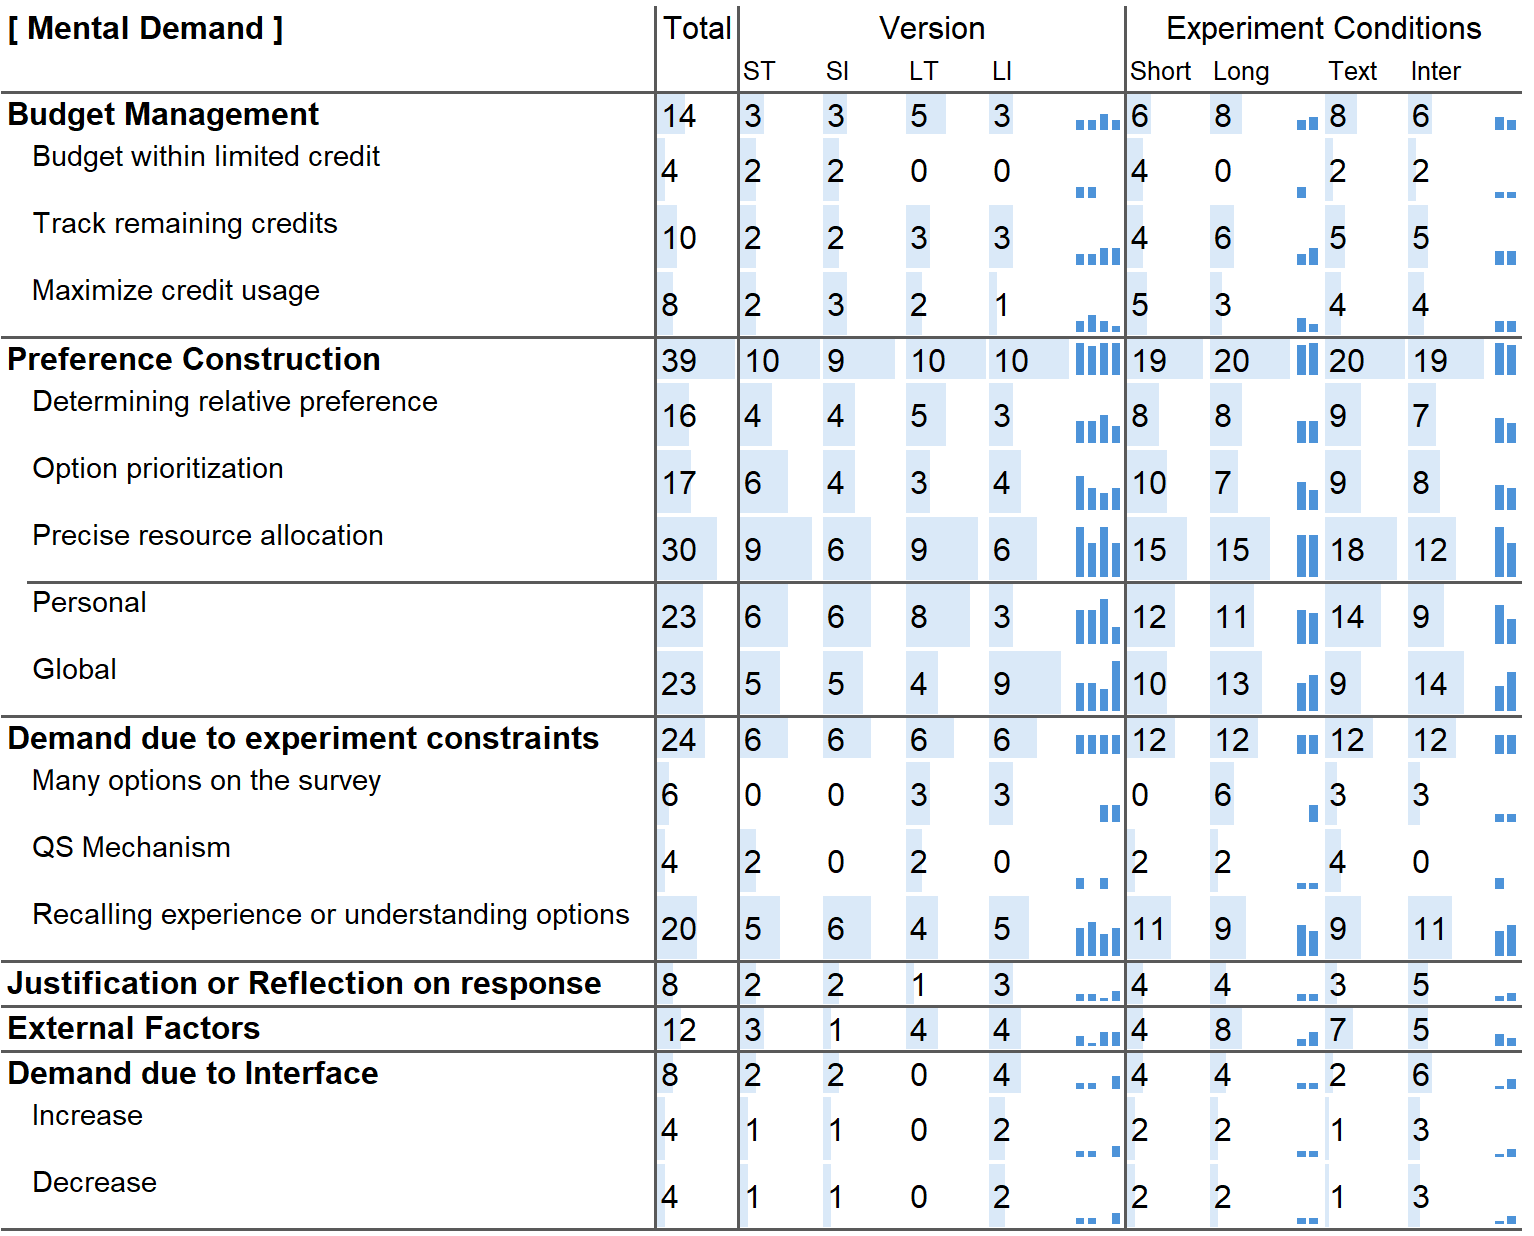
\includegraphics[width=\linewidth]{content/image/cog/mental_table.png}
\end{table}

\subsection{Sources of Physical Demand} 
\label{apdx:physical}
Physical demand refers to the physical effort required to complete a task, such as physical exertion or movement. Most participants reported minimal physical demand~($N=32$), reflected in the low NASA-TLX physical demand scores~(Figure~\ref{apdxfig:physical_cog_score}). Notably, $11$ out of $20$ participants who used the two-phase interface mentioned physical demand from using the mouse, reflecting their increased interaction with the interface. This is further supported by the raw NASA-TLX physical demand scores~(Figure~\ref{apdxfig:physical_cog_score}), which show a significant visual difference between short and long two-phase interfaces as well as between text and two-phase interfaces in long surveys. Table~\ref{apdx:physical_table} presents all the relevant codes across experiment groups.


\begin{table}[h]
    \caption{Physical Demand Causes: Most participants expressed little or no physical demand. Results reflected that participants in the long two-phase interface required more actions, hence the higher mention of mouse usage as a source.}
    \Description{A table showing physical challenges experienced by participants, including Reading, Mouse, Vertical Screen, and None/Little physical effort, with sparklines and percentage bars visualizing the data trends. Data is split across four interface versions (ST, SI, LT, LI) and experiment conditions (Short, Long, Text, Inter). The Mouse category has the highest counts, with trends clearly visible via sparklines and bars, while Reading and Vertical Screen challenges have lower values. The None/Little row shows participants reporting minimal physical effort with percentage bars illustrating the distribution.}
    \label{apdx:physical_table}
    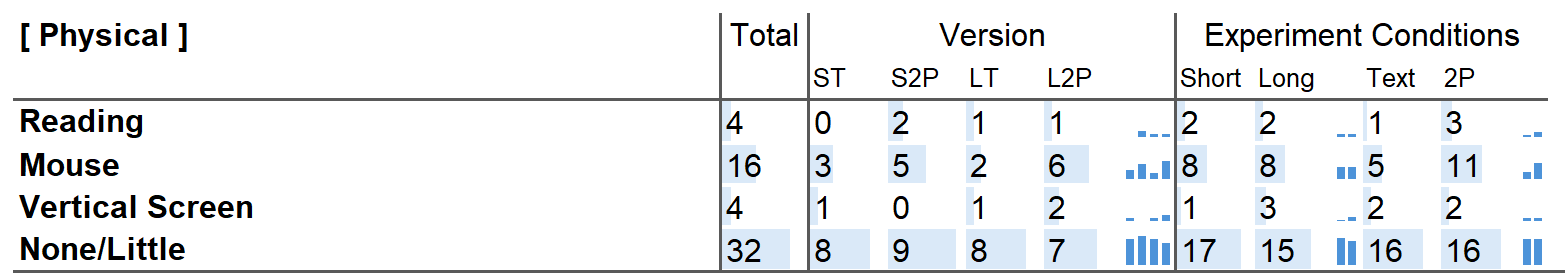
\includegraphics[width=\linewidth]{content/image/cog/physical_table.png}
\end{table}

\begin{figure}[h]
    \begin{minipage}[t]{0.45\textwidth}
        \centering
        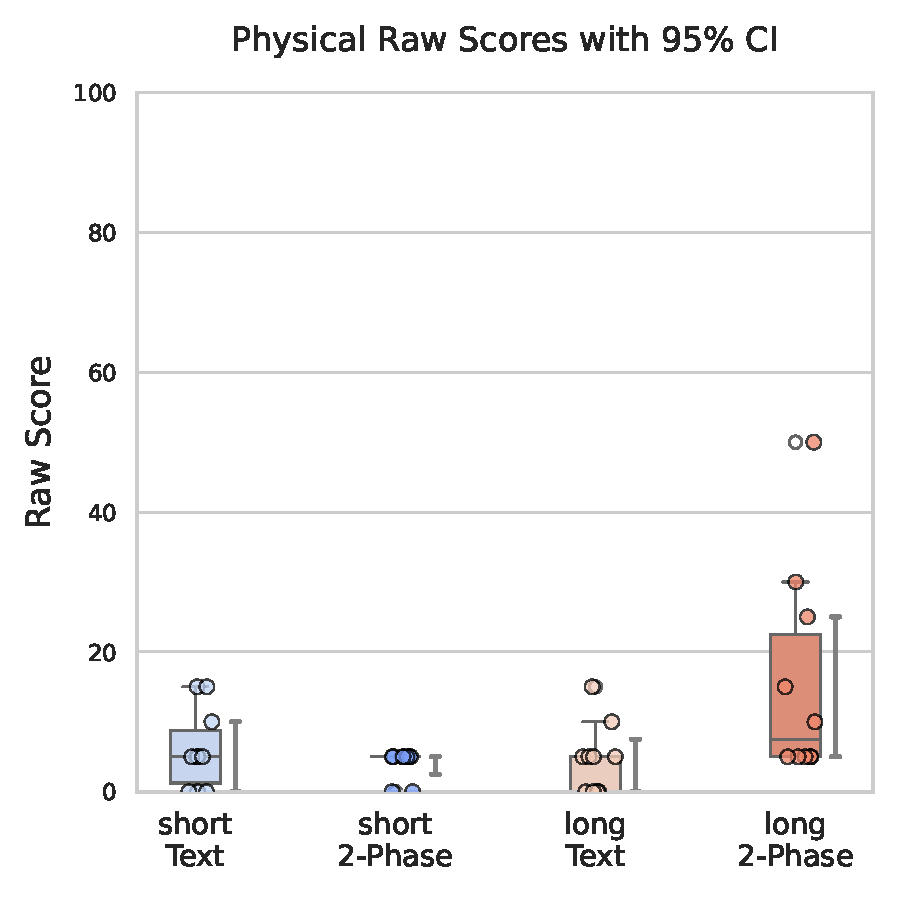
\includegraphics[width=\textwidth, trim=0 13 0 13, clip]{content/image/cog/Physical_scores.pdf}
        \captionsetup{width=0.9\textwidth, justification=justified}
        \caption{Physical Demand Raw Score: Participants other than the long two-phase interface reported minimal physical demand. The long two-phase interface had the highest physical demand, likely due to increased mouse clicks and extended time spent looking at the vertical screen.}
        \Description{A box plot showing the distribution of physical raw scores across four interface versions: Short Text, Short 2-Phase, Long Text, and Long 2-Phase. The y-axis represents the raw score ranging from 0 to 100. The box plots include individual data points, a central line for the median, and whiskers indicating the 95\% confidence interval. The Short Text, Short 2-Phase, and Long Text interfaces show minimal physical demand, with scores clustered below 20. The Long 2-Phase interface exhibits higher physical demand, with a few scores scattered up to around 60.}

        \label{apdxfig:physical_cog_score}
    \end{minipage}
    \hfill
    \begin{minipage}[t]{0.45\textwidth}
        \centering
        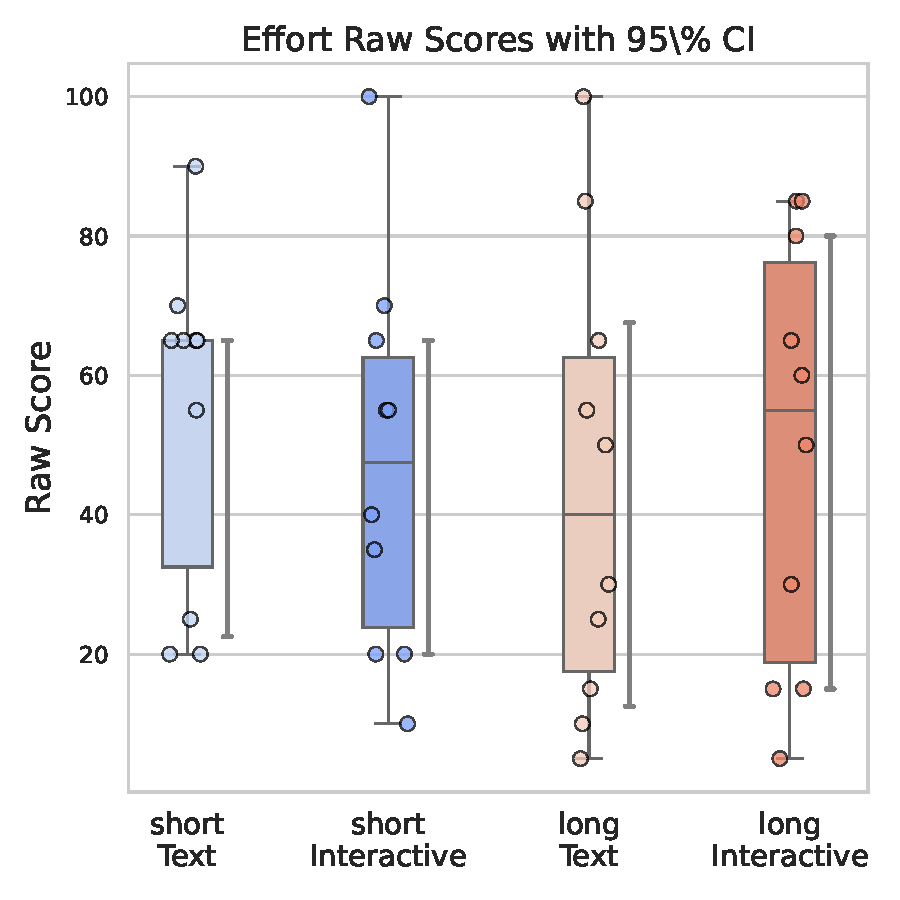
\includegraphics[width=\textwidth, trim=0 13 0 13, clip]{content/image/cog/Effort_scores.pdf}
        \captionsetup{width=0.9\textwidth, justification=justified} % Adjust the width to match the image width
        \caption{Effort Raw Score: Effort scores shows indifference across groups.}
        \Description{A box plot showing the distribution of effort raw scores across four interface versions: Short Text, Short 2-Phase, Long Text, and Long 2-Phase. The y-axis represents the raw score ranging from 0 to 100. Each box plot includes individual data points, a central line indicating the median, and whiskers representing the 95\% confidence interval. The Long 2-Phase interface shows the widest range of effort scores, while the other interfaces display more compact distributions. Data points are scattered within and outside the whiskers, reflecting variability in effort scores across the groups.}
        \label{apdxfig:effort_cog_score}
    \end{minipage}
\end{figure}

% ============================================= %
\begin{table}[h]
    \caption{Effort Sources: Participants using the text interface focused more on operational tasks, while those using the two-phase interface focused more on strategic planning.}
    \Description{A table summarizing participant effort as Operational and Strategic (personal and global), with data visualized using sparklines and percentage bars. The table is split into four versions (ST, SI, LT, LI) and experiment conditions (Short, Long, Text, Inter), with counts and corresponding bars for each category. The operational effort shows participants managing tasks, while the strategic effort captures balancing personal preferences with societal concerns. Sparklines highlight trends across different conditions. A None/Little/A bit row shows participants exerting minimal effort, visualized with bars.}

    \label{apdx:effort_table}
    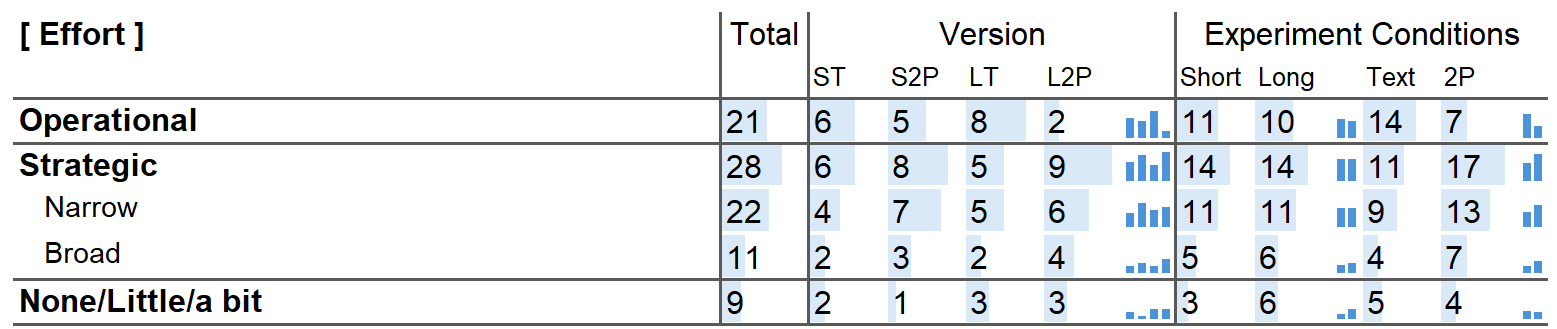
\includegraphics[width=\linewidth]{content/image/cog/effort_table.png}
\end{table}

%\vspace{5pt}
% \begin{tldrbox}
%    \faKey~\textbf{Key Differences:} First, participants in the text interface associated effort with operational tasks more often than participants from the two-phase interface. Conversely, participants in the two-phase interface cited more sources from strategic planning than those in the text interface. We observed that participants experienced effort when considering a comprehensive view while using the two-phase interface.
   
%    %Effort sources varied between operational~\textit{Operational Tasks} and~\textit{Strategic Planning}. Participants using the text interface focused on operational tasks, while those using the two-phase interface engaged in strategic planning. This shows that the two-phase interface spurs deeper, more critical thinking.
% \end{tldrbox}

\subsection{Source of Effort}
\label{apdx:effort}
Effort refers to how hard participants felt they worked to achieve the level of performance they did. Since effort includes both mental and physical resource intensity, refer to \Cref{sec:mental} and \Cref{apdx:physical} for definitions. Raw NASA-TLX effort scores~(Figure~\ref{apdxfig:effort_cog_score}) showed a similar spread across experiment groups, the qualitative analysis showed more distinction that participants using the two-phase interface considered options more comprehensively and felt less effort on completing operational tasks, similar to what we found on mental demands~(Section \ref{sec:mental}). Table~\ref{apdx:effort_table} contains codes.

\subsubsection{Effort Source \#1: Operational Tasks} $14$ of the $20$ participants using the text interface mentioned Operational Tasks as effort sources, compared to $7$ using the two-phase interface, with the lowest mention by the long two-phase interface group~($N=2$). Quotes below illustrated participants putting in effort to manipulate the interface.
\begin{displayquote}
I wanted to bump up~(an option) maybe to 4 or <option> to 5 and realize I couldn't.~\bracketellipsis that would be effort came in of how do I want to really rearrange this to make it~(the budget spending) maximize?

\noindent \hfill -- S029, short text interface
\end{displayquote}
\begin{displayquote}
So it was like it was very~\ldots I have to put a lot of effort in terms of you know~\ldots think about each dimension that if I give one credit to <option name> whether it will affect my credits on <another option name>. \noindent\hfill -- S005, long text interface
\end{displayquote}

\subsubsection{Effort Source \#2: Strategic Planning} Different from Operational Tasks, $11$ participants in the text interface compared to $17$ participants described strategic planning as sources of effort, with almost all participants~($N=9$) from the long two-phase interface. We further categorize strategic planning into \textit{narrow} and \textit{broad} scopes as we did for mental demand~\cref{sec:mental}. Participants using the two-phase interface~($N=7$) had nearly mentioned double~($N=4$) times regarding global strategies. For example:

\begin{displayquote}
And really the bulk of the effort was how to rank order these~(options) and allocate the resources behind the upvotes so that I can accurately depict what I want~\ldots say, a committee to focus on and allocate actual fungible resources, too. \noindent \hfill -- S019, long two-phase interface
\end{displayquote}


% However, qualitative analysis revealed that participants using the text interface experienced more effort focused on operational tasks~(i.e., completing specific tasks). In contrast, participants using the two-phase interface experienced more effort focused on strategic planning~(planning a strategy to complete tasks). Specifically, those using the two-phase interface engaged in global strategic planning, considering options comprehensively and beyond the immediate task. This contrasts with text interface participants, who concentrated more on operational tasks and narrower strategic planning. This finding reinforces that cognitive load sources differ between interfaces, with two-phase interfaces fostering deeper, more critical thinking.

%Both examples show considerations beyond personal experiences, including outcomes or social values. Nearly twice as many participants using the two-phase interface~($N=7$) mentioned global strategic efforts compared to the text interface~($N=4$). Overall, more participants using the two-phase interface~($N=17$) reported sources of strategic effort compared to those using text-based interfaces~($N=11$).

%\subsubsection{Takeaway: Two-phase interface spurs more strategic effort from participants}
%Effort is a realization of mental demand through physical actions. Since participants experienced little physical demand, the sources of effort reflected how individuals translated their mental demand into efforts. The raw NASA-TLX effort scores~(Figure~\ref{fig:effort_cog_score}) showed a similar spread across experiment groups, akin to mental demand. However, qualitative analysis revealed that participants using the text interface experienced more effort focused on operational tasks~(i.e., completing specific tasks). In contrast, participants using the two-phase interface experienced more effort focused on strategic planning~(planning a strategy to complete tasks). Specifically, those using the two-phase interface engaged in global strategic planning, considering options comprehensively and beyond the immediate task. This contrasts with text interface participants, who concentrated more on operational tasks and narrower strategic planning. This finding reinforces that cognitive load sources differ between interfaces, with two-phase interfaces fostering deeper, more critical thinking.

%\begin{wrapfigure}{r}{0.45\textwidth} % Adjust the width as needed
%    \centering
%    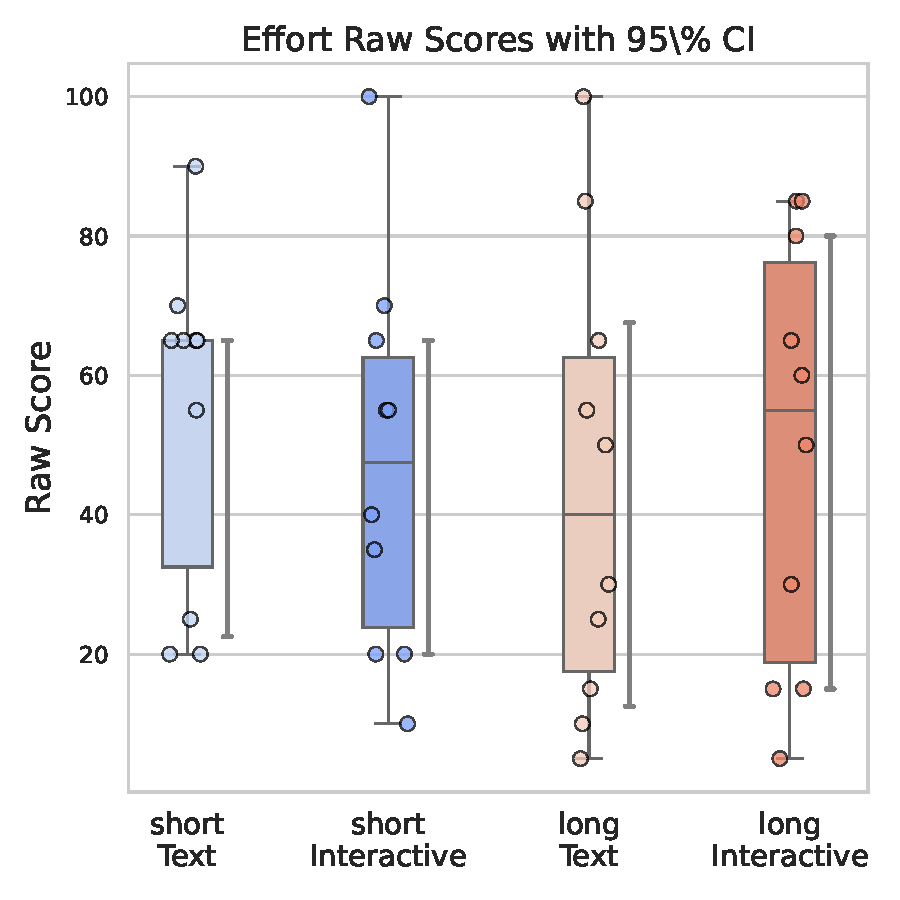
\includegraphics[width=0.45\textwidth, trim=0 13 0 13, clip]{content/image/cog/Effort_scores.pdf}
%    \captionsetup{width=0.40\textwidth, justification=justified} % Adjust the width to match the image width
 %   \caption{Effort Raw Score: Effort scores shows indifference across groups.}
  %  \label{fig:effort_cog_score}
%\end{wrapfigure}


%\subsubsection{Effort Source: Strategic Planning}
%Strategic planning is similar to strategic budget management mentioned under mental demand. Unlike operational tasks, strategic planning involves higher-level strategies to complete the survey. We categorize two distinct types of planning: \textit{personal} and \textit{global}. \textit{Personal strategic planning} involves translating preferences onto the survey without considering broader values or beliefs. For example:

%\begin{displayquote}
%~\bracketellipsis having that prior experience and being able to quickly link it to a tangible thing that I've experienced in my personal life.

%\noindent \hfill -- S032, short text interface
%\end{displayquote}

%\begin{displayquote}
%And really the bulk of the effort was how to rank order these~(options) and allocate the resources behind the upvotes so that I can accurately depict what I want~\ldots say, a committee to focus on and allocate actual fungible resources, too. 

%\noindent \hfill -- S019, long two-phase interface
%\end{displayquote}

%Participants using the two-phase interface~($N=13$) mentioned personal strategic planning slightly more than those using the text interface%\end{displayquote}

%\begin{displayquote}
%Hey, even though I don't really like this idea. But what if they're important? They sort of kind of deserve some attention~\ldots that's why I think I have the effort here.

%\noindent \hfill -- S037, long two-phase interface
%\end{displayquote}
% ============================================= %
\begin{table}[ht]
    \caption{Performance Causes: Most causes are shared across experiment conditions. We provided qualitative interpretations of their own performance assessments.}
    \Description{A table detailing participant performance across Operational Action (budget control, preference reflection, limited resources), Social Responsibility (decision maker, outcome uncertainty), and Performance Assessment (did their best, feel good, good enough). The table includes sparklines and percentage bars to visualize the distribution of performance data across four interface versions (ST, SI, LT, LI) and experiment conditions (Short, Long, Text, Inter). Operational action and social responsibility are visually represented, with sparklines highlighting performance trends.}

    \label{tbl:physical}
    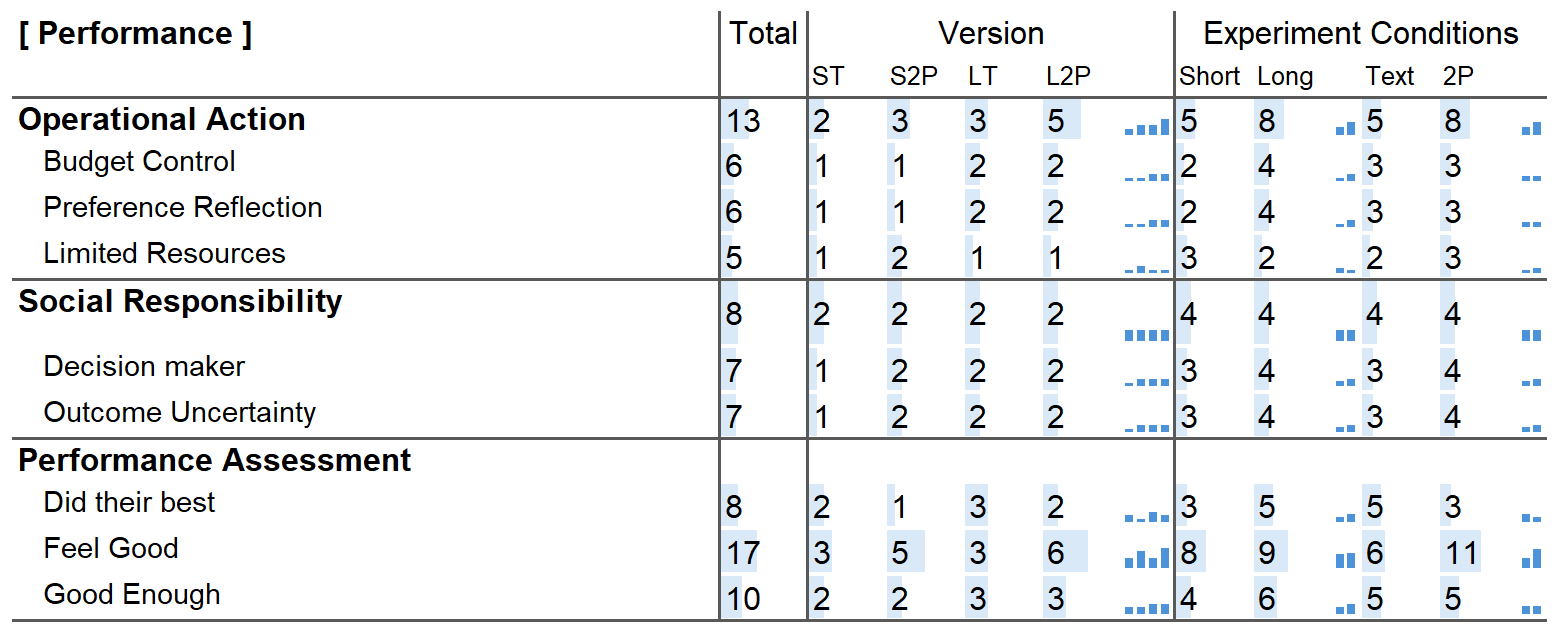
\includegraphics[width=0.95\linewidth]{content/image/cog/perf_table.png}
\end{table}

\subsection{Source from Performance}
\label{apdx:performance}

Performance refers to a person's perception of their success in completing a task. Lower values mean good perceived performance; higher values mean poor perceived performance. We found minimal qualitative differences between experiment groups regarding factors influencing perceived performance. Two influencing factors emerged: \textit{Operational Actions} and \textit{Social Responsibility}. Despite most participants reporting positively on their performance, nuances exist in how different groups interpret their performance.

\begin{wrapfigure}{r}{0.45\textwidth} % Wrap figure on the right
    \centering
    \adjustbox{valign=t}{
        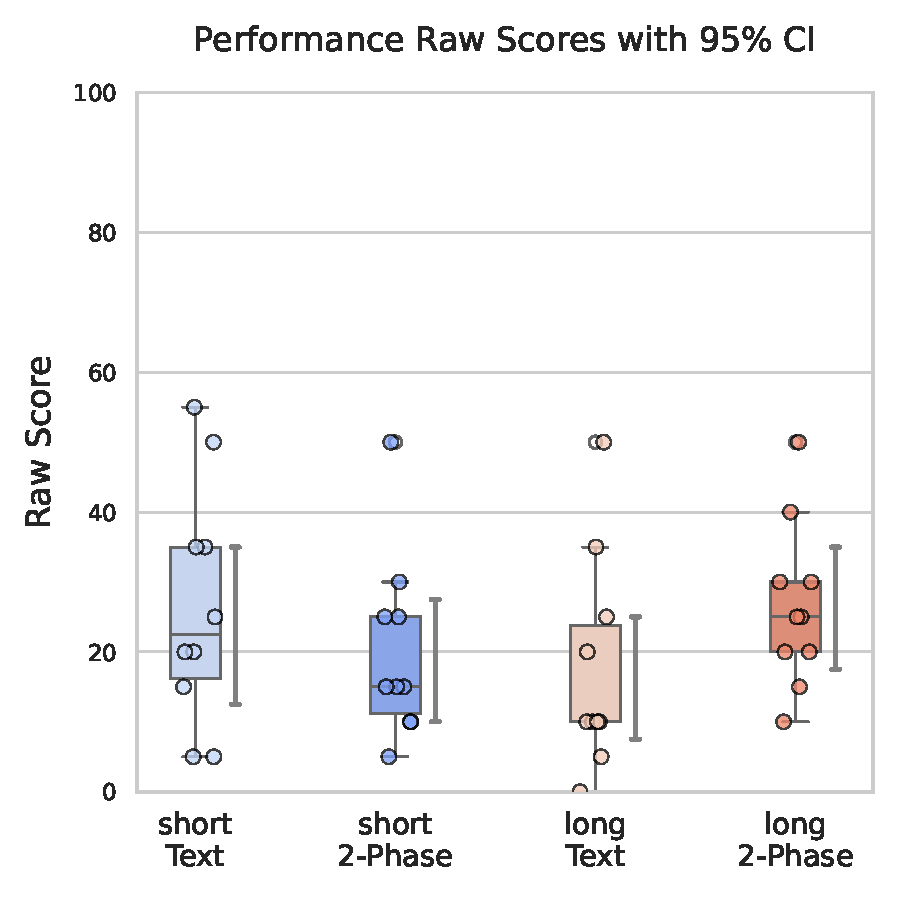
\includegraphics[width=\linewidth, trim=0 13 0 13, clip]{content/image/cog/Performance_scores.pdf}
    }
    \captionsetup{width=0.9\linewidth, justification=justified}
    \caption{Performance Demand Raw Score: Participants showed indifferent performance raw scores across experiment conditions, all trending toward satisfactory.}
    \Description{A box plot displaying the distribution of performance raw scores across four interface versions: Short Text, Short 2-Phase, Long Text, and Long 2-Phase. The y-axis represents raw scores ranging from 0 to 100. Each box plot includes individual data points, a central line for the median, and whiskers representing the 95\% confidence interval. The performance scores appear relatively low across all conditions, with medians hovering between 20 and 40.}

    \label{fig:performance_cog_score}
\end{wrapfigure}

\subsubsection{Operational Actions}
Operational actions, like the theme presented in temporal demand, refer to specific, executable procedures participants perform in the survey. This could involve: pressure to spend all credits or stay within budget~($N=6$), fears that final vote choices did not reflect true preferences($N=5$), or concerns that they had finished the task inefficiently~($N=6$).


\subsubsection{Social Responsibility}
Social responsibility-based concerns around performance came up when participants reflected on how their final vote counts would be perceived by others~(\smallquote{S041}{I don't want people to think that I just like don't care about <ethnicity> people at all}) or influence real-world decision-making~(\smallquote{S027}{Some of these things might \ldots have outcomes that I didn't foresee}).

All groups cited social responsibility as source to evaluate effort. Raw NASA-TLX scores~(Figure~\ref{fig:performance_cog_score}) show participants had indistinguishable performance scores. This aligns with the interview results where most participants felt positive about their final submission. 

To dig deeper, we also analyzed participants' language when they described their performance. Expressions like ``good enough'' may be indicative of satisficing behaviors -- our results suggest participants are satisfied at similar rates regardless of the interface. 1/4 of the participants in the text interface expressed ``done their best,'' referring to exhausting their effort. Participants who used a two-phase interface were generally more positive about their final outcome -- they were twice as likely to report "feeling good" about their final results~($N=11$ v.s. $N=6$).


\subsection{Temporal Demand}
Table~\ref{apdx:temporal_table} lists all the mental demand codes.
\label{apdx:temporal_table}
\begin{table}[ht]
    \caption{Temporal Demand Sources: Decision-making and Operational Tasks are the main causes. Participants framed their decision-making sources differently.}
    \Description{A table categorizing temporal challenges across Budget Management, Decision Making (affirmative and negative), and Operational (task completion, efficiency). The data includes sparklines and percentage bars to visualize patterns across four versions (ST, SI, LT, LI) and experiment conditions (Short, Long, Text, Inter). Affirmative decision-making shows higher values than negative decision-making, with percentage bars indicating the relative distribution. Temporal operational tasks show consistent effort across conditions, as reflected in the sparklines.}

    \label{tbl:temporal}
    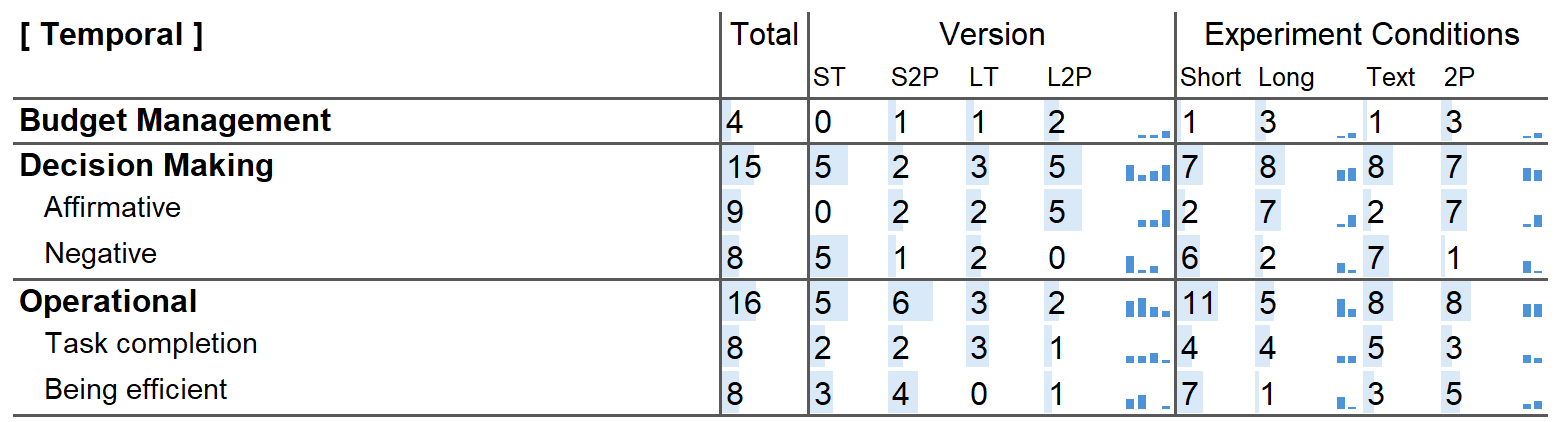
\includegraphics[width=\linewidth]{content/image/cog/temporal_table.png}
\end{table}

\subsection{Frustration}
Table~\ref{apdx:frus_table} lists all the mental demand codes.
\label{apdx:frus_table}
\begin{table}[ht]
    \caption{Frustration Sources: Frustration comes from different levels of strategic operations or operational tasks.}
    \Description{A table with sparklines showing frustration categories: Strategic (higher-level and lower-level) and Operational, across four versions (ST, SI, LT, LI) and experiment conditions (Short, Long, Text, Inter). The table includes sparklines and percentage bars alongside the numerical counts to visually represent the data distribution across conditions. Strategic frustration is divided into higher-level and lower-level conflicts between personal preference and broader societal values. Operational frustration includes challenges such as credit management, adhering to the quadratic mechanism, making decisions, and understanding options. A final row captures participants reporting None/Little frustration, also visualized with percentage bars.}

    \label{tbl:fustration}
    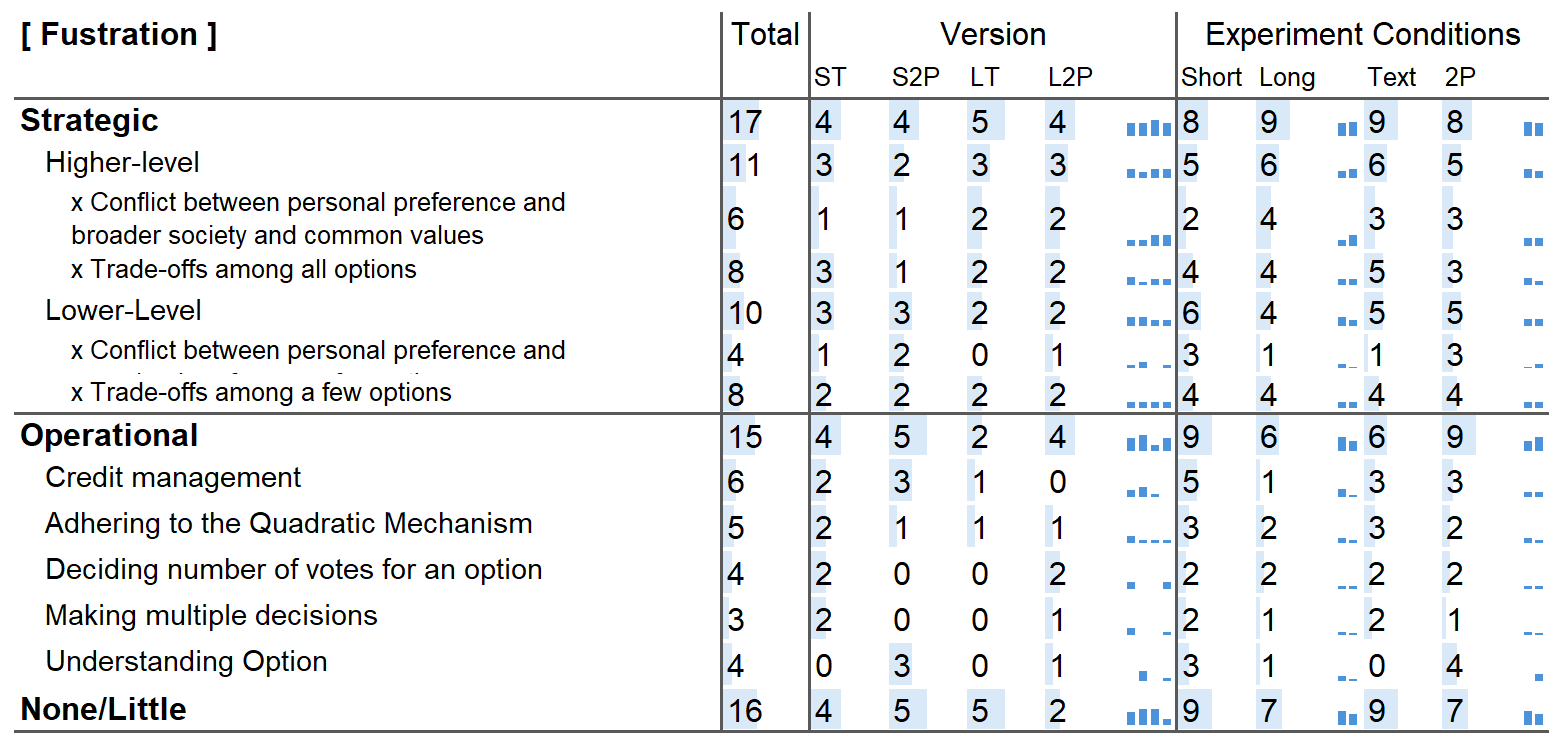
\includegraphics[width=\linewidth]{content/image/cog/fustration_table.png}
\end{table}

% TODO: Need to check the reflective thinking part a bit. I **think** there are differences but it is unclear, need to go back to raw code.

% \begin{figure}[h]
%     \begin{minipage}[t]{0.45\textwidth}
%         \centering
%         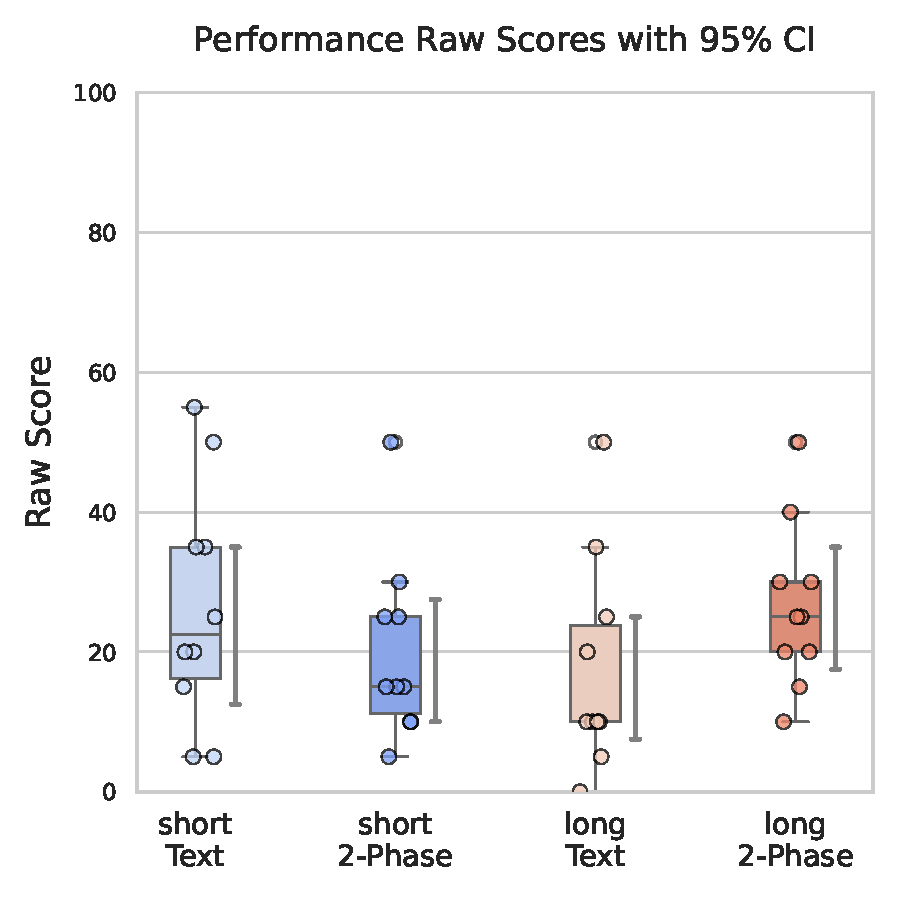
\includegraphics[width=\textwidth, trim=0 13 0 13, clip]{content/image/cog/Performance_scores.pdf}
%         \captionsetup{width=\textwidth, justification=justified} % Adjust the width to match the image width
%         \caption{Performance Demand Raw Score: Participants showed indifferent performance raw scores across experiment conditions, all trending toward satisfactory.}
%         \label{fig:performance_cog_score}
%     \end{minipage}
%     \hfill
%     \begin{minipage}[t]{0.45\textwidth}
%        \centering
%        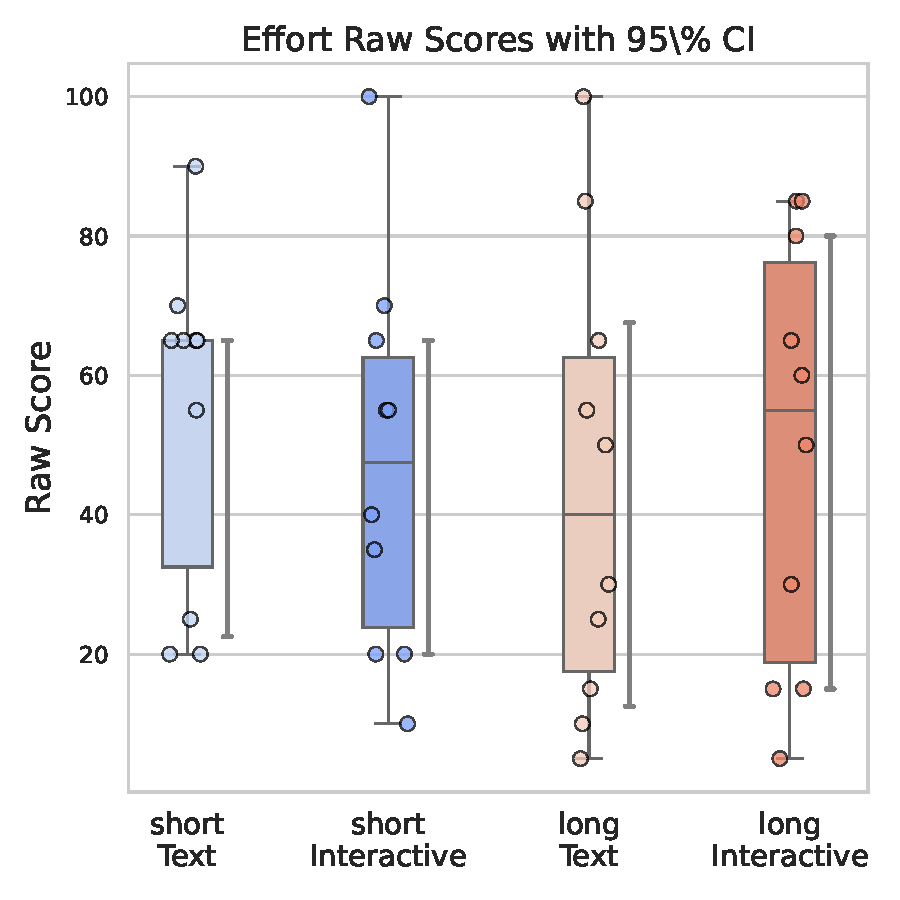
\includegraphics[width=\textwidth, trim=0 13 0 13, clip]{content/image/cog/Effort_scores.pdf}
%        \captionsetup{width=\textwidth, justification=justified} % Adjust the width to match the image width
%        \caption{Effort Raw Score: Effort scores show indifference across groups.}
%        \label{fig:effort_cog_score}
%     \end{minipage}
% \end{figure}


\newpage
\section{Additional voting behavior data}
\label{apdx:additional_results_behavior}
The reason why we decided to focus on the percentage of remaining credits comes from prior literature `scarcity frames value'~\cite{Shah2015a}, a driver that makes researchers believe makes quadratic voting more accurate~\cite{chengCanShowWhat2021}. We did not follow ~\textcite{quarfoot2017quadratic} in counting accumulated votes over time due to varying total times across individuals.

In this section, we complement the main text, showing a few additional figures. Figure~\ref{apdxfig:voting_all} follows the main text, showing all the voting actions over the remaining credit for the four experiment conditions. Here we see two distinct patterns between the short survey and the long survey in terms of participant behaviors. In long surveys, participants exhibited more actions both when the budget was abundant and when it began to run out. This pattern was more pronounced with the long two-phase interface. This difference is why we further focused on the long QS group.

\begin{figure}[ht]
    \centering
    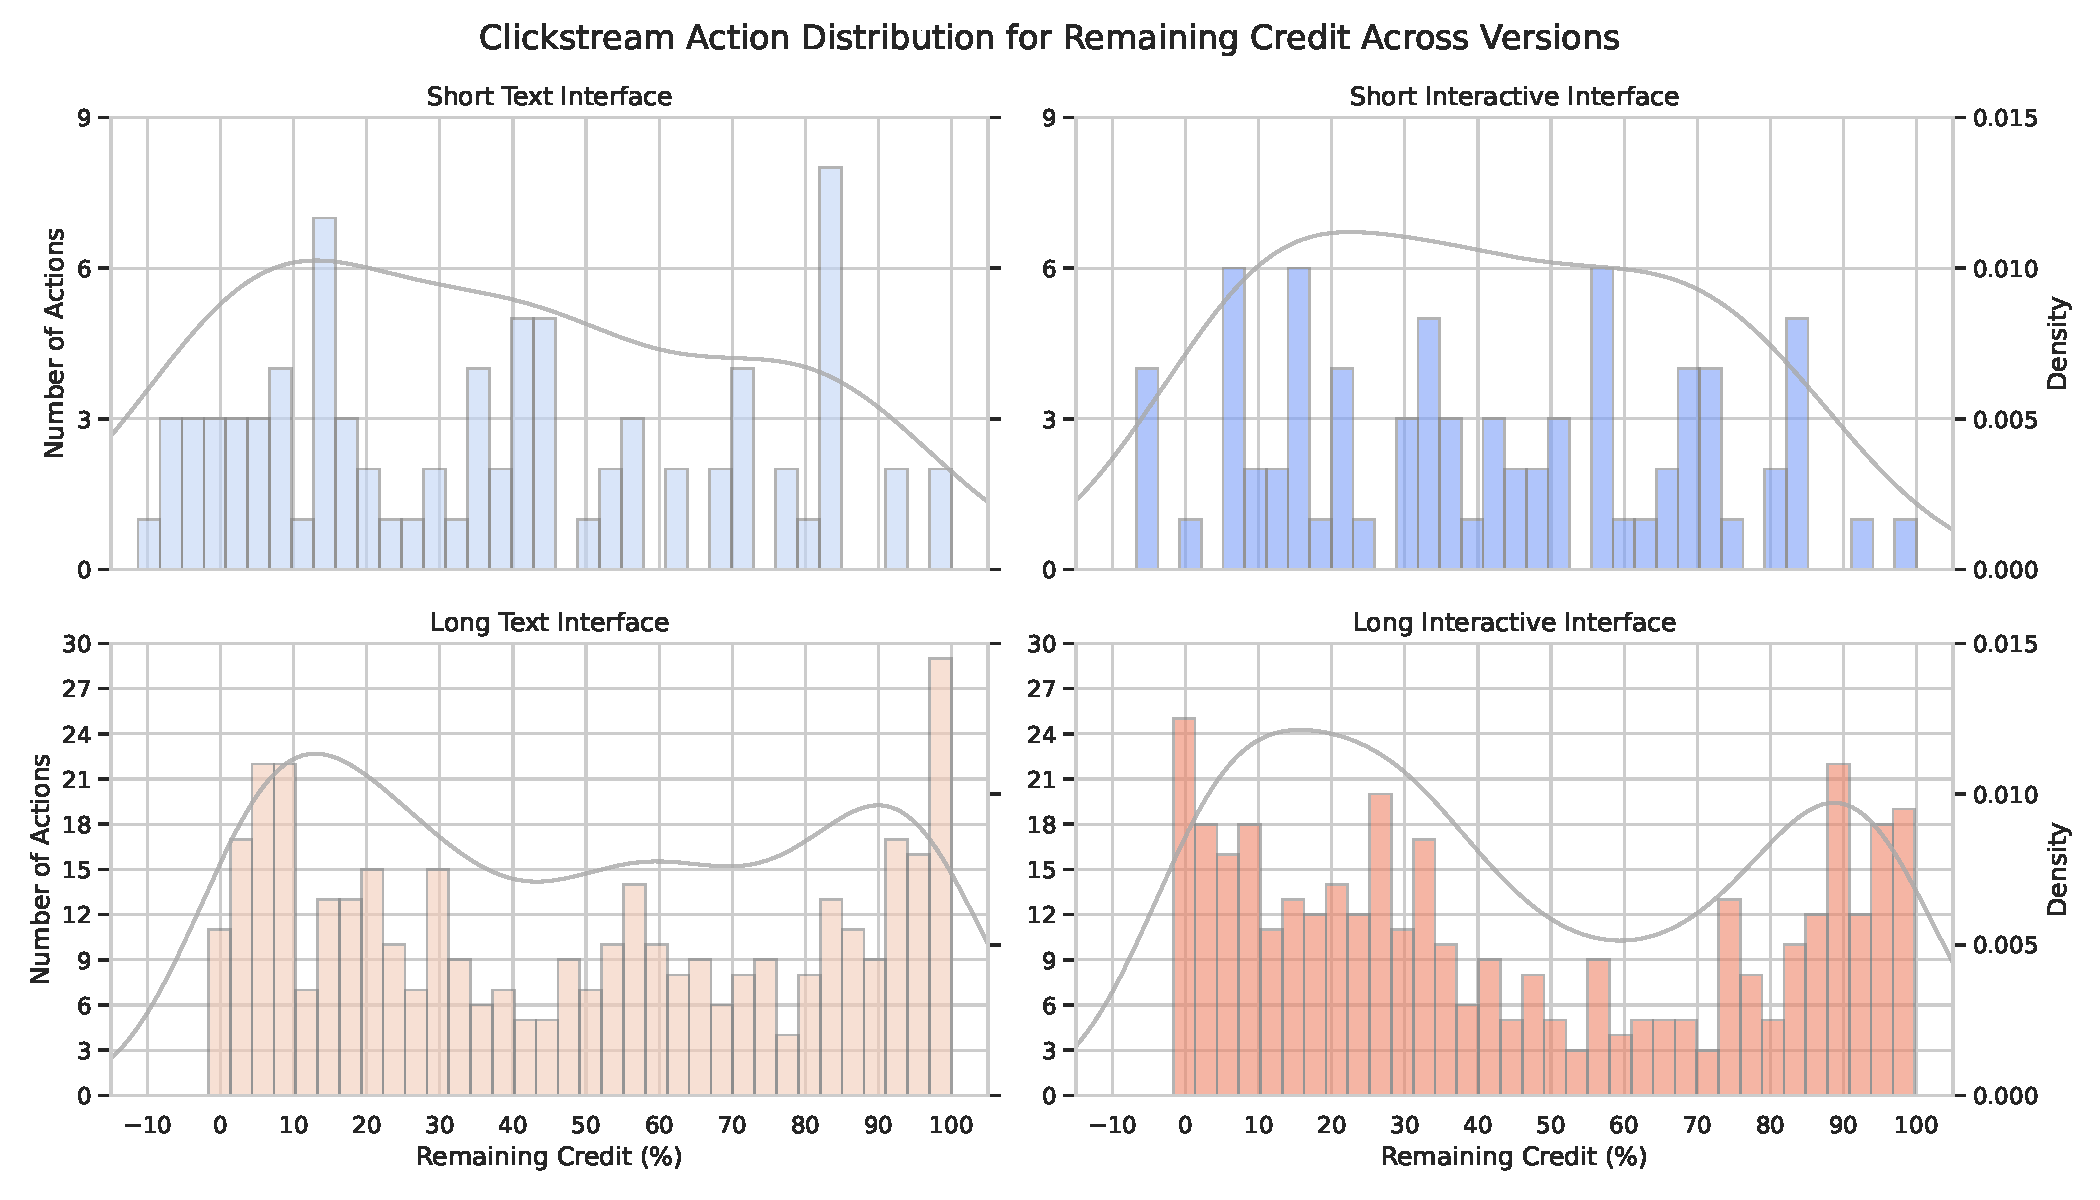
\includegraphics[width=\textwidth]{content/image/results/clickstream_action_distribution.pdf}
    \caption{This plot counts the number of voting actions when there are $x$ percentages of credits remaining. A KDE plot is provided to help better understand the action distribution.}
    \Description{A four-panel histogram showing the number of voting actions across remaining credit percentages for four interface versions: Short Text, Short 2-Phase, Long Text, and Long 2-Phase. Each panel displays the number of actions on the y-axis and remaining credit on the x-axis, with an overlaid KDE curve representing density. In the top panels (Short Text and Short 2-Phase), actions are distributed relatively evenly, with small peaks around 10-20\% and 50\% remaining credit. The KDE curves show minor fluctuations. In the bottom panels (Long Text and Long 2-Phase), there are more pronounced peaks at 0-10\% and 100\% remaining credit, with broader distributions and smoother KDE curves indicating denser actions around these areas. The Long Text and Long 2-Phase interfaces exhibit more actions overall compared to the Short Text and Short 2-Phase interfaces.}
    \label{apdxfig:voting_all}
\end{figure}

\begin{figure}[ht]
    \centering
    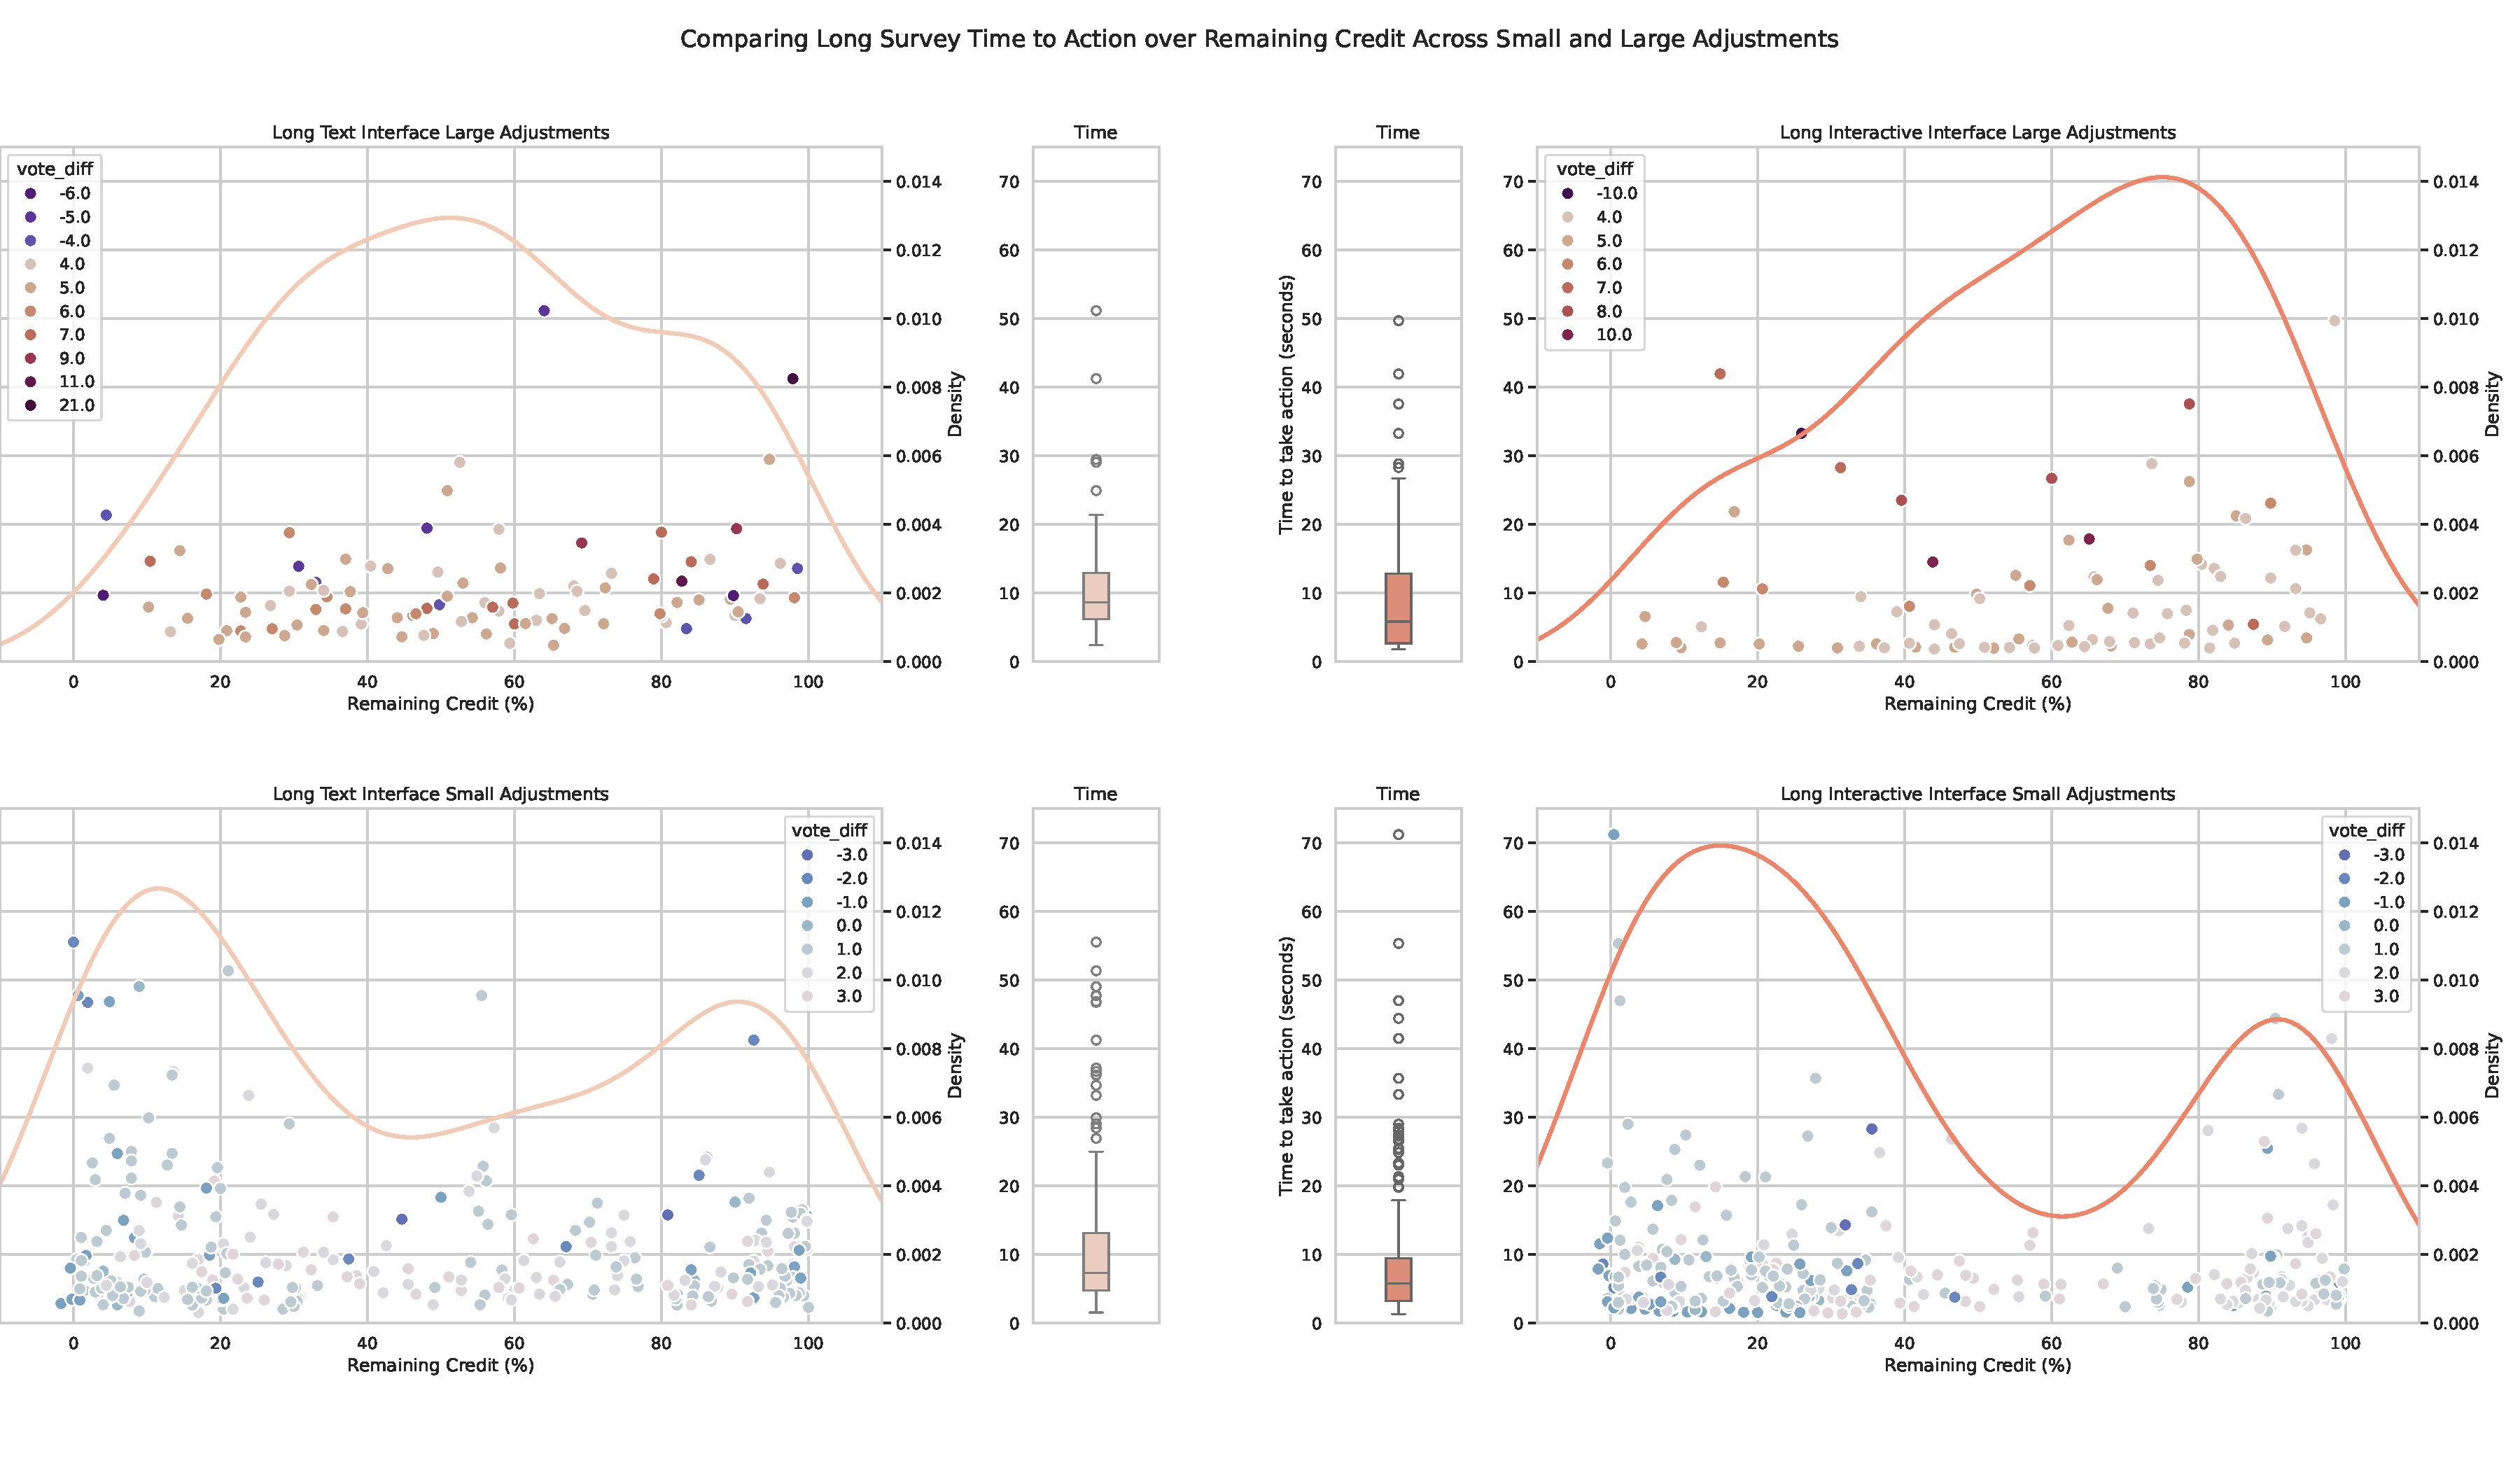
\includegraphics[width=\textwidth]{content/image/results/combined_density_plots.pdf}
    \caption{This plot further separates participants' interaction behavior based on the number of votes participants adjusted. We observed a bimodal interaction pattern across long QS when small vote adjustments are made.}
    \Description{A four-panel plot comparing the time to take action in seconds over remaining credit percentages for large and small vote adjustments in the Long Text and Long 2-Phase interfaces. Each panel includes scattered points and an overlaid KDE curve. The top left panel shows large vote adjustments for the Long Text interface, with peaks in the KDE curve around 20\% and 80\% remaining credit. The top right panel shows large vote adjustments for the Long 2-Phase interface, with two peaks in the KDE curve around 10\% and 100\%. The bottom left panel shows small vote adjustments for the Long Text interface, with scattered points and peaks in the KDE curve around 10\% and 90\%. The bottom right panel shows small vote adjustments for the Long 2-Phase interface, with a KDE curve peaking around 10\% and 100\% remaining credit. Box plots on the right side of each panel summarize the distribution of time taken to adjust votes for each interface.}    
    \label{apdxfig:voting_v3_v4}
\end{figure}

In addition to the small adjustment plots presented in Figure~\ref{fig:small_clicks}, Figure~\ref{apdxfig:voting_v3_v4} presents the comparison between when participants make small or large vote adjustments at different budget levels. Revisiting the KDE curve in the second row in Figure~\ref{apdxfig:voting_all} and the curve of the second row in Figure~\ref{apdxfig:voting_v3_v4} show a stronger bimodal distribution for small vote adjustments across interfaces. In fact, the bimodal distribution is more pronounced in the two-phase interface. This suggests that participants make small adjustments both at the beginning and toward the end of the QS. However, the two-phase interface shows more frequent and faster edits towards the end. In comparison, participants also made more large vote adjustments early on that spread more equally compared to the text interface. This indicates that participants had a clearer idea of how to distribute their credits across the options.

\section{Demographic Breakdown}
\label{apdx:demo}
TODO

\section{Voting Interfaces and Response Format}

Research in the marketing and research communities focusing on survey and questionnaire design, usability, and interactions examines the influence of presentation styles and `response format.'~\textcite{weijtersExtremityHorizontalVertical2021} demonstrated that horizontal distances between options are more influential than vertical distances, with the latter recommended for reduced bias. Slider bars, which operate on a drag-and-drop principle, show lower mean scores and higher nonresponse rates compared to buttons, indicating they are more prone to bias and difficult to use. In contrast, visual analog scales that operate on a point-and-click principle perform better~\cite{toepoelSlidersVisualAnalogue2018}. These studies show how even small design changes can have a large impact on usability, highlighting the importance of designing interfaces that prioritize human-centered interaction rather than focusing solely on functionality.

Voting interfaces are a specialized type of survey interface that not only elicit individual choices but often have consequential impacts. For example, the butterfly ballot, an atypical design, may have influenced the outcome of the 2000 U.S. Presidential Election~\cite{wandButterflyDidIt2001}. Research has shown that ballot interfaces can significantly influence democratic processes~\cite{engstrom2020politics, chisnellDemocracyDesignProblem2016, DesigningUsableBallots2015}. Several studies also highlighted how voting interface designs shift voter decisions~\cite{engstrom2020politics}, reduce usability errors~\cite{quesenberyOpinionGoodDesign2020, everettElectronicVotingMachines2008}, or improve interaction~\cite{leeUniversalDesignBallot2016, summers2014making, dawkinsPrimeIIIInnovative2009, gilbertAnomalyDetectionElectronic2013, conradElectronicVotingEliminates2009}. We provide more details to these voting interfaces in the Appendix~\ref{apdx:relatedVoting}.

From the QV implementations, response format literature, and voting interfaces, we identified how interfaces significantly influence respondent behavior, decision accuracy, and cognitive load. While these systems are functional, they lack the human-centered design needed to reduce cognitive load and make them truly usable, rather than simply operable. These burdens are especially problematic for complex systems like QS, where high cognitive demands may deter researchers and users alike. Developing effective, human-centered interfaces for QS could enhance usability, reduce cognitive overload, and increase adoption in both research and practical applications.
